\chapter{Úvod}

V~dnešní době, kdy lidé jsou zvyklí na větší pohodlí než kdysi, narůstá i počet chytrých domácností.
Chytré domácnosti by měly usnadnit život lidem, okolí, i dokonce celé planetě.
Když se řekne chytrá domácnost, může se někomu například vybavit jakýsi robot, který vám uklidí, či dokonce přinese nákup.
Chytrá domácnost může být jakkoliv chytrá, dokonce se může podobat i domácnostem z~různých sci-fi filmů.
Můžeme si uvést příklad z~každodenního života většiny z~nás.
Večer přijdete domů s~těžkým nákupem, musíte vyndat z~kapsy klíče (se štěstím, že jsouprávě v~kapse), pracně otevřít, položit nákup, rozsvítit na chodbě, zhasnout na chodbě,
rozsvítit v~kuchyni atd.
Teď si představte, že se blížíte ke dveřím, kamera rozpozná váš obličej, otevřou se dveře, rozsvítí se světla, vozík odveze váš nákup k~lednici a Vy si nemusíte ničeho všímat.

Chytrá domácnost má ale i další výhody a to především při úspoře energie.
Úspora energie hraje v~dnešní době velice důležitou roli.
Při výrobě elektrické energie se vyprodukuje mnoho skleníkových plynů, které zatěžují životní prostředí.
Chytrá domácnost může rapidně snížit produkci těchto plynů.
Největším odběratelem elektrické energii v~domácnostech jsou především různá topná telěsa, ať už v~podobě elektrického topení, nebo ohřívačů vody, dále různá osvětlení apod.
Tito největší odběratelé pracují většinou celý den a komplexně pro celý dům, avšak určité změny by byly velice přínosné, např. vytápění pouze obývaných prostor,
snižování intenzity osvětlení podle okolní intenzity světla, různé akce vykonané podle aktuálního času apod.
Podle mého názoru se chytré domácnosti dostanou do popředí, na trhu v~oblasti informačních technologiích, velice rychle.
Je samozřejmé, že chytré domácnosti a chytré zařízení již existují.
Ovšem nastává problém, kdy tato zařízení jsou velice drahá a výrobce, většinou, podporuje pouze svá zařízení a je téměř nemožné sestavit chytrou domácnost z~různých komponentů od různých výrobců.

Cílem této práce je vytvořit kompletní řešení chytré domácnosti, které bude levné a připojená různá zařízení budou mezi sebou komunikovat bez ohledu na výrobce.
Dále hlavním rysem tohoto projektu je poskytnutní přístupnosti k~domácnosti. Tento systém je navržen tak, aby mohl být nasazen v~cloudu a být přístupný pro tisíce uživatelů zároveň. Vyžaduje se určitá robustnost systému a hlavně bezpečnost.
Někteří uživatelé však cloudové služby nepodporují a bezpečnost je u~nich na prvním místě. Pro tento případ je systém navržen tak, aby mohl běžet na samostatném mini počítači pouze v~rámci domácnosti. Dalším cílem práce je poskytnout uživateli
intuitivní rozhraní pro snadné zprovoznění chytré domácnosti a následné správě domácnosti.

Práce je rozdělena na několik dalších hlavních částí:
\emph{důležité termíny} (kapitola \ref{terminy}),
\emph{návrh řešení} (kapitola \ref{navrh}),
\emph{použité technologie} (kapitola \ref{pouzite}),
\emph{implementace řešení} (kapitola \ref{implementace}),
\emph{testování} (kapitola \ref{testovani})
a samotný \emph{závěr} (kapitola \ref{zaver}).

\chapter{Důležité termíny}
\label{terminy}

V~této kapitole jsou popsány důležité termíny které jsou nezbytné k~porozumnění zbytku práce.
Asi nejdůležitější je pochopit koncept \emph{IoT}, který je popsán v~podkapitole \ref{terminy:iot}.
V~dalších podkapitolách najdeme stručné vysvětlení pojmu \emph{MCU - neboli mikrokontrolér}(kapitola \ref{terminy:iot}), informace o~různých zařízeních, která jsou obsažena v~implementaci této chytré domácnosti.
Specifičtěji se jedná hlavně o~moduly \emph{ESP} (kapitola \ref{terminy:esp8266}) a mini počítač \emph{Raspberry Pi} (kapitola \ref{terminy:raspberry}).
Komunikace mezi zařízeními probíhá pomocí protokolu \emph{MQTT}, komunikace s~uživatelským rozhraním (dále jako \emph{frontend} nebo \emph{klientská aplikace}) a serverem, kde je obsažena celá business logika (dále \emph{backend}), zajištuje protokol \emph{HTTP}.

\bigskip

\section{IoT - Internet věcí}
\label{terminy:iot}

\emph{IoT} je zkratka pro \emph{\textbf{I}nternet \textbf{o}f \textbf{T}hings}, neboli \emph{Internet věcí}.
V~informatice se jedná o~označení pro síť fyzických zařízení, vozidel, domácích spotřebičů a dalších zařízení, která jsou vybavena elektronikou,
softwarem, senzory, pohyblivými částmi a síťovou konektivitou, která umožňuje těmto zařízením se navzájem propojit a vyměňovat si data.
Každé z~těchto zařízení je jasně identifikovatelné díky implementovanému výpočetnímu systému,
ale přesto je schopno pracovat samostatně v~existující infrastruktuře internetu.~\cite{wiki:iot}

Jak vyplývá z~definice \emph{IoT}, zařízení v~domácnosti jsou propojena (např. přes \emph{switch}, nebo \emph{router}) a navzájem komunikují.
Po síti se posílají data z~různých senzorů a různá zařízení na tato data reagují jiným způsobem.
Data mohou být vyhodnocována přímo daným zařízením, nebo systémem, který je pro zařízení dostupné.
Tento systém může být ve formě distribuované sítě, kde data mohou být vyhodnocována a zasílána i na druhý konec světa.
V~\emph{IoT} velmi často vystupuje \emph{umělá inteligence} (dále jako \emph{AI} - \emph{artificial intelligence}), která může předávat data různým zařízením a vyhodnocovat pomocí neuronových sítí.

\emph{IoT} je využíváno i v~prostředí různých výrobních procesů, či linek.
V~továrnách, kde velké stroje plní svoji práci, mohou také mezi sebou komunikovat dané stroje a rozdělení práce mezi dané stroje může být tímto přístupem velice efektivní.
Stroje rozloží výrobní proces tak efektivně, že všechny stroje jsou zatížené způsobem, který odpovídá požadavkům zavedeným na daný proces.
Amortizace těchto strojů se sníží, a proto i náklady na výrobu jsou nižší.
Stroje mohou mezi sebou komunikovat dokonce i mimo lokální továrny a vyměňovat si data např. o~počtu materiálu, který je přítomen na skladě a opět efektivně přerozdělovat materiál do více skladů a továren.

\newpage

\section{Vestavěný systém}
\label{terminy:vestaveny}

Vestavěný systém, neboli \emph{Embedded system} je hardwarový systém, který je tzv. \emph{microprocessor-based}(založený na mikroprocesoru).
Obsahuje software, který je navržen k~vykonávání určité specifické činnosti buď jako nezávislý systém, nebo jako část většího celku.
Nejvýznamnější komponenta vestavěného systému je integrovaný obvod, který je navržen pro operace, které jsou závislé na reálném čase(dále jako \emph{real-time} systém).~\cite{embedded:info}

K~vestavěnému systému lze připojit mnoho vstupních/výstupních periferních zařízení, které spolupracují s~mikrokontrolérem (více info viz. \ref{terminy:mcu}) obsaženým ve vestavěném systému.
Na obrázku níže je vyznačeno jednoduché schéma, které pojednává o~asociaci mezi vestavěným systémem, vstupních/výstupních zařízení a dalších náležitostí.

Nejdůležitější částí je připojení vstupních zařízení, mezi které může patřit např. klávesnice, tlačítka a různé senzory.
Vestavěný systém pomocí mikrokontroléru vyhodnotí získaná data a přivede na výstup patřičnou hodnotu, odpovídající programovému zpracování dat podle obsaženého softwaru (také označovaný jako \emph{firmware}).
Mezi výstupní zařízení můžeme zahrnout např. různá relé, tranzistory, audio a video výstupy a mnoho dalších.

\begin{figure}[hbt]
  \centering
  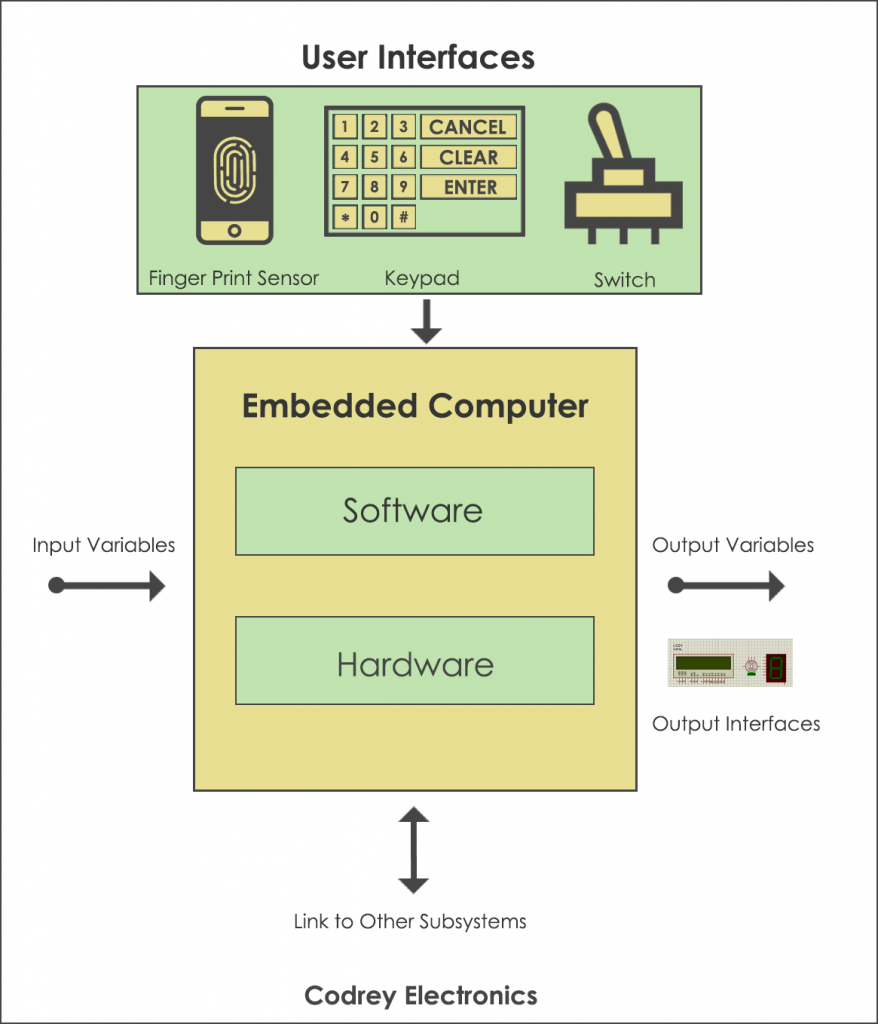
\includegraphics[width=.6 \linewidth]{obrazky-figures/embedded_system.png}
  \caption{
    Koncept vestavěného systému.~\cite{embedded:figure}
  }
  \label{figure:embedded}
\end{figure}

\newpage
\section{MCU - mikrokontrolér}
\label{terminy:mcu}

Mikrokontrolér (zkratka MCU\footnote{\textbf{MCU} - \textbf{M}icro\textbf{C}ontroller \textbf{U}nit}), nebo také jednočipový počítač, je integrovaný obvod, který obsahuje kompletní \emph{mikropočítač}.
Mikrokontroléry jsou velice spolehlivé, kompaktní a proto hojně využívány k~řízení různých elektronických systému, obykle pomocí mikroprocesoru, paměti a různých periferních zařízení.
Tato malá zařízení jsou optimalizována pro vestavěné systémy popsané výše, které potřebují zpracovat interakci s~digitálními, analogovými, nebo elektromechanickými komponentami.

Název pro mikrokontrolér byl velice vhodně zaveden, protože opravdu zdůrazňuje charakteristiku typu daného zařízení. Mikrokontroléry jsou malá zařízení, která dokáží velké věci.
Mikrokontroléry hrají důležitou roli v~technologické budoucnosti. Získavají si velikou oblibu nejen u~různých SW\footnote{\textbf{SW} - software}/HW\footnote{\textbf{HW} - hardware} expertů, ale i studentů a spousty hobby nadšenců.~\cite{mcu:info}
Díky mikroprocesorům lze jednoduše propojit SW nástroj, či aplikaci s~HW komponentami.

Blížící se budoucnost přinese spoustu nových možností v~oblasti miktrokontrolérů a počet zařízení obsahující mikrokontrolér může v~blízké době přesáhnout i několika desítek miliard kusů.
Výkon u~těchto zařízení bude vyšší a velikost menší, což je občas velice důležitý faktor na poli chytrých domácností.
V~chytré domácnosti jsou zařízení sestavena s~pomocí mikrokontroléru, který se stará o~danou specifickou funkci. V~této bakalářské práci jsou především použity mikrokontroléry s~čipem ESP-8266 od firmy \emph{Espressif Systems}
a minipočítač \emph{Raspberry Pi}. Obrázek níže obsahuje odpovídající architekturu skoro každého mikrokontroléru.
Mezi hlavní prvky patří analogově-digitální převodník, čítače, časovače, modul řídící PWM\footnote{\textbf{PWM} - \textbf{P}ulse-\textbf{W}idth \textbf{M}odulation (pulsně šířková modulace).}.

\begin{figure}[hbt]
  \centering
  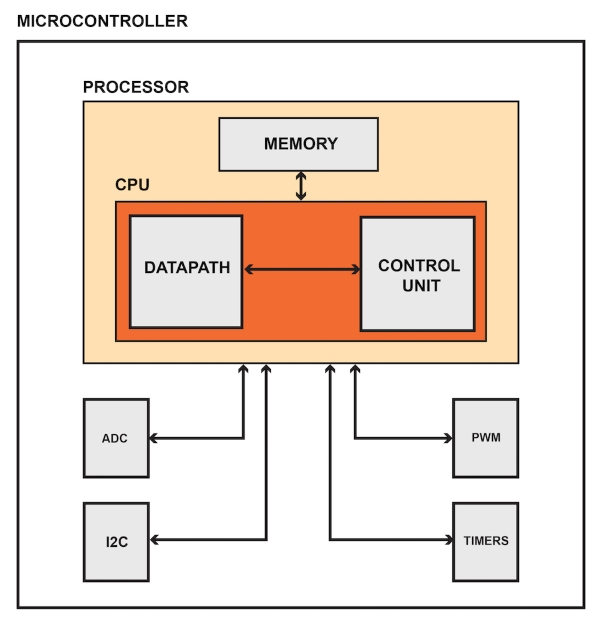
\includegraphics[width=.6 \linewidth]{obrazky-figures/mcu.jpeg}
  \caption{
    Koncept mikrokontroléru.~\cite{mcu:info}
  }
  \label{figure:mcu}
\end{figure}

\newpage

\section{MQTT protokol}
\label{terminy:mqtt}

\emph{MQTT} neboli \emph{Message Queuing Telemetry Transport} protokol je jeden z~nejvýznamnějších komunikačních protokolů IoT zařízení a systémů.
\emph{MQTT} patří do kategorie aplikačních protokolů, kde jeho hlavní předností je malá velikost datové hlavičky a možnost komunikovat v~sítích s~omezenou propustností.
Patří do skupiny \emph{Publish-Subscribe}(dále \emph{Pub-Sub}) protokolů.
Hlavním principem \emph{Pub-Sub} protokolů je výměna zpráv mezi dvěma typy účastníků. První z~nich je tzv. odebíratel(dále \emph{subscriber}),
který se přihlašuje k~odběru zpráv s~daným temátem(dále \emph{topic}).
Subscriber může přijímat několik zpráv s~různými tématy a v~průběhu se od odběru i odhlašovat. Druhým typem je tzv. vydavatel(dále \emph{publisher}), který posílá zprávy do určitého
topicu.~\cite{mqtt:info}

\subsection*{MQTT Broker}
\emph{MQTT Broker} je služba (nebo-li software, který běži v~cloudu, či lokálním PC), která se stará o~rozesílání a spravování zpráv, které různá zařízení posílají.
\emph{MQTT Broker} je prostředník mezi účastníky typu \emph{subscriber} a \emph{publisher}.
Každé zařízení, které chce využívat MQTT protokol a komunikovat s~ostatními zařízeními, musí definovat \emph{URL}\footnote{\textbf{URL} - \textbf{U}niform \textbf{R}esource \textbf{L}ocator (jednotná adresa zdroje)} brokeru, přes který budou dané zprávy procházet.
Jak již bylo řečeno, \emph{MQTT} je \emph{Pub-Sub} protokol, proto když přijde od účastníka typu publisher zpráva ke specifickému topicu, musí se podívat, kdo všechno je přihlášen k~odběru daného topicu a rozeslat všem účastníkům, typu subscriber, danou zprávu.
Každé zařízení může jak přijímat, tak i odesílat zprávy k~danému topicu.~\cite{wiki:mqtt_broker}

\subsection*{Zabezpečení}
V~\emph{IoT} je velice důležitá i bezpečnost a pomocí \emph{MQTT Brokeru} lze dosáhnout určitého bezpečnostního cíle. Je opravdu nevítané, aby se někdo cizí dostal bez autentizace k~odběru vašich
zpráv procházející přes \emph{MQTT Broker} a mohl zasílat zprávy do různých dalších zařízení připojená v~domácnosti.
Útočník tak má šanci kontrolovat celou vaši domácnost. Každý \emph{MQTT Broker} od různých výrobců disponuje různou sadou zabezpečení a vlastností.~\cite{wiki:mqtt_broker}
\newline

Možné typy zabezpečení:
\begin{itemize}
  \item Využívání šifrovaného portu \textbf{8883} namísto nešifrovaného \textbf{1883}
  \item Autentizace pomocí uživatelského jména a hesla
  \item \textbf{TLS}\footnote{\textbf{TLS} - \textbf{T}ransport \textbf{L}ayer \textbf{S}ecurity} připojení
  \item \textbf{OAuth}\footnote{\textbf{OAuth} - Poskytuje autentizační a autorizační správu} správa
\end{itemize}

\newpage
\subsection*{Typy zpráv}
\emph{MQTT} protokol využívá sadu různých typů zpráv pro vlastní běh. Na obrázku \ref{figure:mqtt_flow}lze zahlédnout posloupnost zpráv.~\cite{wiki:mqtt_broker}
Mezi základní typy zpráv u~protokolu MQTT patří:
\begin{itemize}
  \item \textbf{CONNECT} - slouží pro ustanovení připojení
  \item \textbf{CONNACK} - (\emph{Connection acknowledge}) typ zprávy je odezva z~brokeru klientu, který požadoval o~připojení a vytvoří se spojení mezi uzly
  \item \textbf{SUBSCRIBE} - neboli odběr; klient pošle tuto zprávu brokeru na určitý topic u~kterého chce přijímat dané zprávy
  \item \textbf{UNSUBSCRIBE} - slouží k~odhlášení klienta od odebírání zpráv z~určitého topicu
  \item \textbf{PUBLISH} - slouží na publikování zpráv na různý topic (např. zasílání dat ze senzorů)
  \item \textbf{DISCONNECT} - slouží k~odhlášení klienta z~celého systému
\end{itemize}

\begin{figure}[ht]
  \centering
  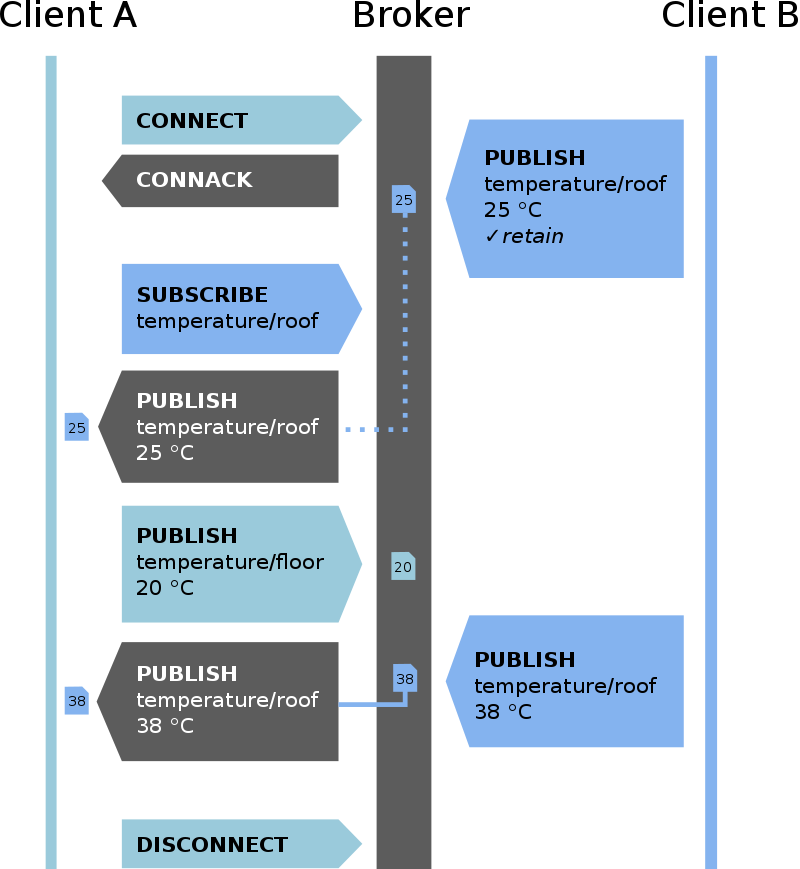
\includegraphics[width=.7 \linewidth]{obrazky-figures/mqtt_flow.png}
  \caption{Posloupnost MQTT zpráv.~\cite{wiki:mqtt}}
  \label{figure:mqtt_flow}
\end{figure}

\newpage
\subsection*{QoS - Kvalita služeb (\emph{Quality of Services})}
Každá zpráva může specifikovat, jakým způsobem bude zajištěna kvalita služeb u~zasílaných zpráv.~\cite{wiki:mqtt_broker}
\begin{itemize}
  \item \textbf{\emph{QoS 1}} - Nejvýše jednou; zpráva je zaslána pouze jednou bez potvrzení.
  \item \textbf{\emph{QoS 2}} - Alespoň jednou; zpráva stále zasílána dokud nedorazí potvrzení o~přijetí.
  \item \textbf{\emph{QoS 3}} - Přesně jednou; zajištění, že přijemce dostane zprávu pouze jednou.
\end{itemize}

\subsection*{MQTT over WebSockets (\emph{MQTT} pomocí protokolu \emph{WebSocket})}
\label{mqtt:websockets}
\emph{MQTT} přes protokol \emph{WebSocket} je technika, kdy se zabalí komunikační protokol \emph{MQTT} do tzv.\emph{WebSocket frame}(WebSocketový rámec).
Tato technika přenosu je hlavně přínosná pro webové aplikace, tudíž pro vše, co běží v~prohlížeči.
Udává se, že s~touto technikou může být jakýkoliv prohlížeč na různých zařízeních plnohodnotný \emph{MQTT klient}.~\cite{mqtt:hivemq}

Protokol \emph{WebSocket} je v~prostředí webových aplikací velmi dlouhou dobu, poskytuje \emph{full-duplex}\footnote{\textbf{Full-duplex} - obousměrný provoz} komunikaci a umožňuje hladký chod \emph{real-time} aplikací.
Pro inicializaci spojení využívá protokol \emph{HTTP}.
Tato technika tak poskytuje optimální způsob komunikace přes \emph{MQTT} protokol u~zařízení a prohlížeče.

\begin{figure}[ht]
  \centering
  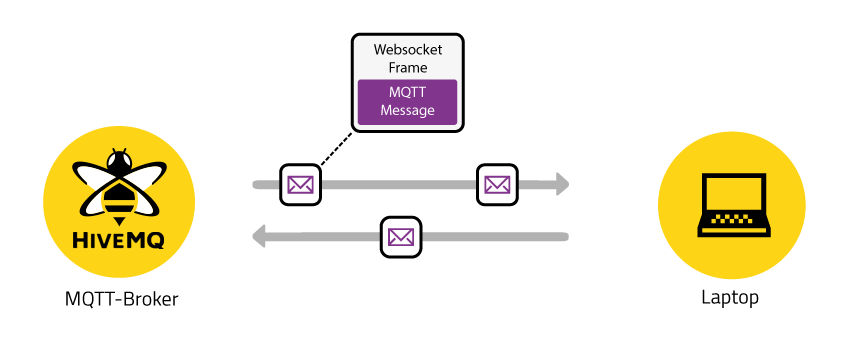
\includegraphics[width=1 \linewidth]{obrazky-figures/mqtt_websocket.png}
  \caption{MQTT over WebSockets.~\cite{mqtt:hivemq}}
  \label{figure:mqtt_websockets}
\end{figure}

\newpage

\section{OIDC}
\label{app_prostredi:oidc}

\begin{figure}[hbt]
  \centering
  
\includegraphics[width=.35 \linewidth]{obrazky-figures/OIDC.png}
  \caption{OIDC logo}
\end{figure}

\textbf{OIDC} nebo-li \emph{OpenID Connect} je autentizační protokol, založený na specifikaci \emph{OAuth 2.0}. Tento protokol využívá služba \emph{KeyCloak}, která je použita v~této bakalářské práci.
\emph{OIDC} protokol využívá \emph{JSON Web Tokens} (dále jako \emph{JWT}), což je formát využit pro reprezentaci ID tokenu.
\emph{OIDC} se hlavně zabývá autentizací uživatelů.
Jeho účelem je poskytnou pouze jeden přihlašovací proces pro více webových stránek.~\cite{terminy:oidc}

\section{JSON}
\label{terminy:json}

\textbf{JSON} nebo-li \textbf{J}ava\textbf{S}cript \textbf{O}bject \textbf{N}otation je formát pro strukturovaná data.
Formát dat se sestavuje podle dvojice \emph{atribut-hodnota} a případně i pole.
\emph{JSON} je nezávislý na programovacích jazycích a je odvozen, jak název vypovídá, z~programovacího jazyka \emph{JavaScript}.
\emph{JSON} je velice rozšířený ve spoustě aplikací, kde téměř všude nahrazuje \emph{XML} formát.

Tento formát zápisu dat je použit v~systému, který popisuje tato bakalářská práce, ve dvou odlišných případech.
První z~nich je při komunikaci s~klientskou aplikací, kde se data zprostředkovávají pomocí daného formátu \emph{JSON}.
V~druhém případě je tento formát použit i u~\emph{MQTT} zpráv zasílaných ze zařízení.
Jedná se hlavně o~zprávy, které se posílají pomocí \emph{MQTT} protokolu na správu zařízení v~domácnosti.
Na obrázku ~\ref{figure:json} je vidět ilustrační zápis dat pomocí \emph{JSON} formátu.

\begin{figure}[hbt]
  \centering
  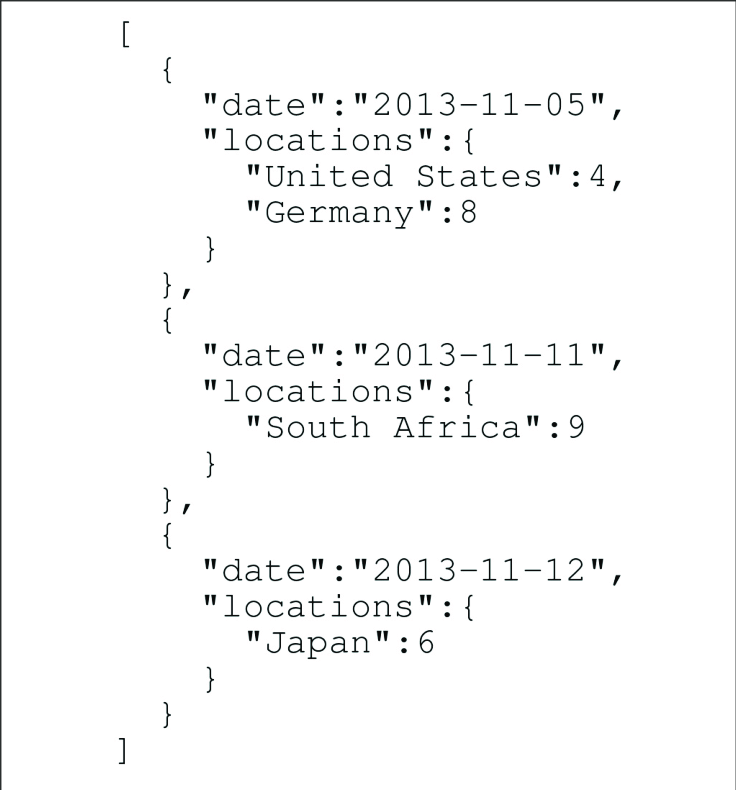
\includegraphics[width=.45 \linewidth]{obrazky-figures/json_example.png}
  \caption{Ukázka \emph{JSON}}
  \label{figure:json}
\end{figure}

\newpage
\section{\emph{RESTful} aplikace}
\label{terminy:restful}
\textbf{\emph{REST}} je akronym\footnote{\textbf{Akronym} - nehláskovaná zkratka} pro \emph{\textbf{RE}presentational \textbf{S}tate \textbf{T}ransfer},
které značí architekturu rozhraní pro distribuované \emph{hypermédia} systémy a byl poprvé prezentován Royem Fieldingem v~jeho disertační práci roku 2000.
\newline
\newline
Jestliže jakékoliv rozhraní chce být považováno za \emph{RESTful}, musí splnit určité podmínky:
\begin{itemize}
  \item \textbf{Klient - Server} - Oddělení uživatelského rozhraní ze serverové části.
        Zlepšení přenositelnosti a škálovatelnosti díky zjednodušení serverových komponentů.
  \item \textbf{Bezstavovost} - Každý požadavek od klienta na server musí obsahovat všechny nezbytné informace k~porozumnění požadavku.
        \emph{Session state}(stav sezení) se celý ukládá pouze u~klienta.
  \item \textbf{Cacheable} (schopný být uložen v~mezipaměti) - Požaduje, aby data v~odpovědi ze serveru byla implicitně, nebo explicitně označena jako \emph{cacheable}, nebo \emph{non-cacheable}.
        Jestliže je odpověď \emph{cacheable}, mezipaměť u~klientské aplikace má právo být znovupoužita později jako odpověď na ekvivalentní požadavek.
  \item \textbf{Jednotné rozhraní} - Použitím principu obecného softwarového inženýrství na rozhraní komponentů se celková architektura systému zjednoduší a zlepší se viditelnost interakcí.
  \item \textbf{Vrstvený systém} - Vrstvený systém umožňuje, aby se architektura skládala z~hierarchických vrstev způsobem omezení chování komponenty tak, že každá komponenta nemůže „vidět“ za nejbližší vrstvu se kterou interagují.
\end{itemize}

Klíčovou abstrakcí informace v~\emph{REST} architektruře je tzv. \emph{resource} (zdroj informací).
Každá informace, která může být pojmenována smí být také považována za zdroj.
\emph{REST} využívá identifikátory zdrojů informací, aby dokázala identifikovat určitý obsah v~interakci mezi komponentami.~\cite{restful:info}
Na obrázku \ref{figure:restful} je popsán tok zpracování požadavků.

\begin{figure}[ht]
  \centering
  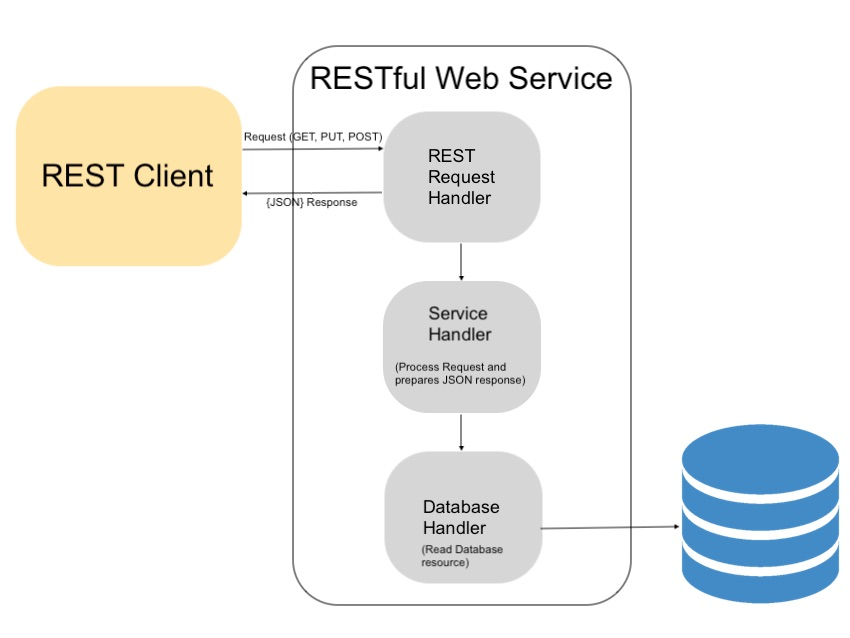
\includegraphics[width=.59 \linewidth]{obrazky-figures/restful.jpg}
  \caption{MQTT over WebSockets}
  \label{figure:restful}
\end{figure}

\chapter{Současný stav a návrh řešení}
\label{navrh}

V~této kapitole je shrnut současný stav řešení chytré domácnosti od nejvýznamnějších firem, které se zabývají tímto tématem a samotný návrh řešení, který by měl danou problematiku vyřešit.
Jak již bylo popsáno v~úvodu, největším úskalím řešení chytré domácnosti je celková cena a kompatibilita se zařízeními od různých výrobců.

V~kapitole \ref{navrh:existujici} jsou popsány existující řešení chytré domácnosti od různých firem a v~kapitole \ref{navrh:reseni} vlastní řešení problému a schopnost dosažení požadovaných cílů.

\section*{Existující řešení}
\label{navrh:existujici}

Kompletních řešení chytré domácnosti existuje v~dnešní době už opravdu nepřeberné množství. Podle mého názoru se postupem let dostane do popředí ještě více \emph{IoT} zařízení a systémů kompletní chytré domácnosti.
Už v~dnešní době spousta obrovských IT firem, mezi které patří např. \emph{Samsung}, \emph{LG}, \emph{Apple} a \emph{Google}, vyvíjí takové systémy.

Například firma \emph{Samsung} představila na trh produkty s~názvem \emph{SmartThings}, které lze využít pro sestavení chytré domácnosti.
Hlavním prvkem, který potřebujete, je tzv. \emph{Hub}, který slouží jako mozek celého systému.
U~svých zařízení většinou využívají pro komunikaci protokol zvaný \emph{Zigbee}, který se řadí do tzv.\emph{ad-hoc}\footnote{\textbf{ad-hoc} - decentralizovaná bezdrátová síť} sítí.
Signály ze zařízení dosahují vzdálenosti 10 až 20 metrů.
\emph{Samsung} se pyšní tím, že jejich zařízení jsou kompatibilní s~více než 100 zařízeními od různých výrobců.
Ale naneštěstí je jejich cena obrovská.

Lze si to představit na jednoduchém příkladu u~chytrého tlačítka od firmy \emph{Samsung}.
Dané tlačítko se vyznačuje tím, že dokáže po nastavení ovládat několik světel současně, spotřebiče, apod.
Tlačítko se v~průměru prodává za nějakých 15\$, což je v~přepočtu něco okolo 380kč.
Tlačítko, které dokáže sadu podobných, dokonce i stejných úkonů, lze sestrojit pro můj vlastní návrh chytré domácnosti asi za cenu okolo 30kč.

Dalším příkladem může být chytrá zásuvka, kterou \emph{Samsung} prodává za cenu blízkou 35\$, což je v~přepočtu asi 880kč a ve své vlastní domácnosti lze sestrojit podobný kus asi za 60kč.
Samozřejmě lze brát v~úvahu i to, že \emph{Samsung} zaručuje kvalitu a dlouhodobou spolehlivost svých zařízení, využívá odlišný protokol, ale cena, podle mého názoru, je až přehnaně vysoká.

\newpage

\section*{Obecný návrh řešení}
\label{navrh:reseni}

Návrh vlastního řešení systému chytré domácnosti je poněkud komplikovanější záležitost díky své rozmanitosti.
Vývojář tak musí být obeznámen s~technologiemi a principy z~různých odvětví aplikačního vývoje.
Systém chytré domácnosti by měl disponovat velikou škálou možností a být jednoduše škálovatelný.
Pro návrh takového systému je potřeba v~první řadě vytvořit analýzu požadavků.
\newline
\newline
Hlavní aspekty, které by měly být splněny:
\begin{itemize}
  \item \textbf{Cena pořízení} - Cena za kompletní systém i jednotlivé komponenty.
  \item \textbf{Zabezpečený systém} - Na všech dostupných úrovních (server, databáze, klientská aplikace, zařízení, přenos dat).
  \item \textbf{Intuitivnost a přístupnost} ovládacích prvků
  \item \textbf{Jednoduchost} - Vytvoření domácnosti a inicializování/připojení zařízení i příliš \textbf{netechnicky zdatným uživatelem}.
  \item \textbf{Sdílení domácnosti} - Schopnost sdílet domácnost s~více uživateli.
  \item \textbf{Autorizace uživatelů v~domácnosti} - Každý uživatel v~různých domácnostech může mít různá přístupová práva.
  \item \textbf{Dostupnost} - Dostupnost systému jak v~případě pouze lokální síťě, tak i s~pomocí cloudových služeb.
  \item \textbf{Použitelnost} - Schopnost systému obstarávat několik tisíc uživatelů zároveň.
  \item \textbf{Customizace\footnote{\textbf{Customizace} - úprava dle požadavků uživatele} zařízení} - Přidávání/odebírání schopností zařízení jednoduchým způsobem.
\end{itemize}
Jak již bylo řečeno, když na návrh systému chytré domácnosti je pouze jeden vývojář, musí se orientovat v~rozmanité sféře technologií, návrhových vzorů apod.
V~dnešní době jsou tyto typy vývojářů označovány jako \emph{Full Stack Developers}, kteří vyvíjí \emph{backend}, tak i \emph{frontend} část aplikace.

V~kapitole \ref{navrh:backend} bude detailněji popsán \textbf{návrh serverové(\emph{backend}) části} systému, která je nejspíše nejkomplikovanější a nedůležitější ze všech odvětví této bakalářské práce.
Dále v~kapitole \ref{navrh:databaze} lze nalézt popis \textbf{návrhu relační databáze} a související věci.
V~kapitole \ref{navrh:frontend} je \textbf{návrh klientské aplikace}(\emph{frontend}), kde hlavním jádrem věci je rozložení a vzhled stránky.
Samozřejmě je zde i popis struktury uložení stavu aplikace a operací provádených na pozadí.
V~poslední kapitole \ref{navrh:hardware} je \textbf{návrh HW zařízení}, struktura programu.
\newpage

Na obrázku \ref{figure:architektura} je graficky znázorněna architektura navrhovaného systému.
Architektura obsahuje server, \emph{MQTT} broker, autentizační/autorizační službu, databázi, klientské aplikace a HW zařízení.
Služby, které budou nasazeny v~cloudu, či v~lokální síti na minipočítači jsou vyznačeny ve žluté části obrázku.
V~zelené části obrázku jsou vyznačeny klientské aplikaci a ve fialové části samotná \emph{HW} zařízení.
Server komunikuje s~\emph{MQTT brokerem} pomocí komunikačnícho protokolu \emph{MQTT}, kde server je další \emph{MQTT klient}(detailně popsáno v~\ref{navrh:backend}).
Server dále komunikuje s~klientskou aplikací (v~zelené části obrázku) pomocí protokolu \emph{HTTP}, která posílá požadavky na server.
Klientská aplikace se serverem dále komunikují s~příslušnou autentizační/autorizační službou.

\begin{figure}[hbt]
  \centering
  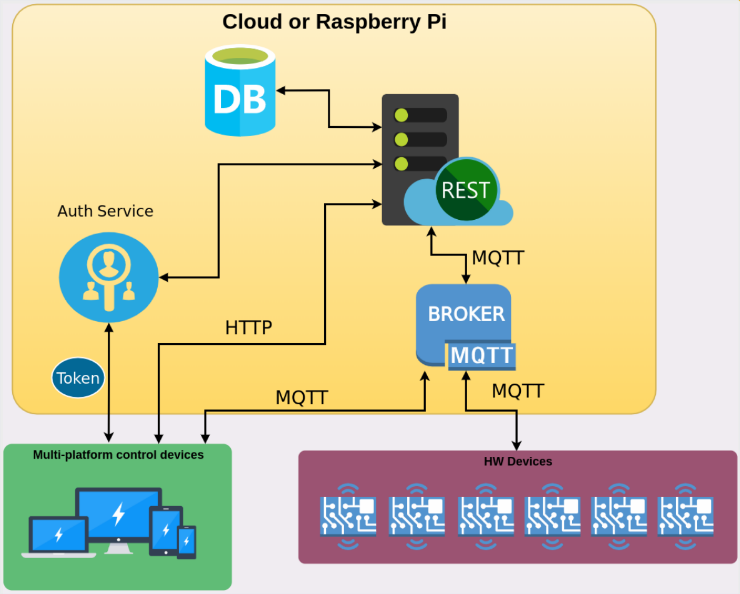
\includegraphics[width=0.8 \linewidth]{obrazky-figures/navrh.png}
  \caption{Základní architektura systému}
  \label{figure:architektura}
\end{figure}

\section{Návrh serverové části}
\label{navrh:backend}
Z~hlediska vývoje aplikací je z~mého pohledu tato část práce nejkomplikovanější a zároveň nejobtížnejší.
Vývojář musí mít dobrý přehled o~technologiích, návrhových vzorech a mnoho dalšího, které lze vhodně aplikovat na danou aplikaci.
Struktura programu této části by měla být sestrojena přehledně a takovým stylem, aby se dala jednoduše rozšiřovat.
Požadavky na aplikaci se mohou velice rychle měnit a vývojář musí dokázat bez většího úsilí implementovat tyto změny.

Serverová část(dále jako \emph{Server}) aplikace se stará o~požadavky, které klientská aplikace, potažmo zařízení, posílá na daný server.
Dále se také zabývá samotnou logikou celého systému, vykonáváním požadavků na databázi, poskytnutím výpočetních sil pro složitější operace a požadavky od zařízení v~domácnosti.
Vytváří rozhraní, ke kterému může přistupovat spousta klientských aplikací a spravovat tak celý management systému chytré domácnosti.

Jedná se tak o~jádro celého systému.
Hlavním úkolem této \emph{backend} aplikace je zprostředkovat služby pro zařízení chytré domácnosti a pro připojení do systému.
Ukládá důležité hodnoty ze zařízení, co se týče stavů výstupních zařízení a poslední hodnoty vstupních zařízení, aby byly stále dostupné při připojení klientské aplikace.
Klientské aplikace vytváří požadavky na danou \emph{backend} aplikaci a získávají tázaná data.
Tato aplikace je vytvořena robustnějším způsobem, aby byla schopna obstarávat požadavky několika tisíců uživatelů.
K~dané aplikaci se váže i otázka bezpečnosti.

Uživatel se musí autentizovat v~daném systému, aby bylo možno identifikovat přihlášeného uživatele a s~tím související autorizační práva na různé zdroje informací.

Mezi velikou škálou programovacích jazyků, které jsou vhodné na vývoj serverových aplikací, jsem si vybral programovací jazyk \emph{Java},
který se v~popularitě těchto technologií drží na předních místech. Programovací jazyk \emph{Java} je objektově orientovaný jazyk, který se velkým způsobem zasadil do vývoje enterprise aplikací.
Jazyk \emph{Java} disponuje rozsáhlým ekosystémem a existuje spoustu výborných frameworků.

Rozhodl jsem se, že serverová část bude sestrojena jako \emph{RESTful}(podrobněji viz. \ref{terminy:restful}) webová služba komunikující nad protokolem \emph{HTTP},
kde u~serveru nebude žádné uživatelské rozhraní, ale pouze programové, známe jako API\footnote{\textbf{API} - \textbf{A}pplication \textbf{P}rogramming \textbf{I}nterface (rozhraní pro programování aplikací)}.
Server poskytne \emph{API}, které využívají klientské aplikace, nebo další služby pro komunikaci se serverem.
Server je bezstavový, což znamená, že si server neukládá stav o~požadavcích a každý požadavek je přijímán stejně, bez jakýchkoli priorit, či upřednostnění díky danému stavu uživatele v~systému.

\subsection*{Zabezpečení}
\label{backend:bezpecnost}
Každý uživatel, který pošle požadavek na server, musí být autentizován.
Server je asociován s~autentizační službou a při každém požadavku na server přepošle tzv. \emph{token}\footnote{\textbf{Token} - žeton pro přístup ke zdrojům informací} autentizační službě
a ta vyhodnotí, zda je uživatel autentizován, potažmo autorizován získat informace z~daného endpointu\footnote{\textbf{Endpoint} - HTTP path (cesta požadavku definována pomocí API)}.
Pokud uživatel není autentizován a nevlastní žádaný \emph{token}, musí poslat požadavek na autorizační službu s~danými \emph{credentials}\footnote{\textbf{Credentials} - poveření v~různých formách (heslo, PIN, OTP, biometrika,...)},
kde získá daný token pro přístup ke zdrojům informací serveru. Token je zasílán v~\emph{HTTP} hlavičce v~atributu \emph{Authorization}.

O~autorizaci se stará přímo server, který ověří u~dané autentizační služby, zda je uživatel autentizován a poté ověří zda má dostatečná práva na zisk informací z~daného zdroje.
Pokud uživatel není autentizován a není přesměrován na stránku autentizační služby, vrací se \emph{HTTP} response\footnote{\textbf{Response} - odpověď na požadavek ze serveru} kód s~číslem 401, který se označuje jako \emph{Unauthorized}(neoprávněný).
Uživatel který není autorizován k~získání informací dostane odpověď ze serveru s~kódem 403, který značí \emph{Forbidden}(zamítnuto).

Server vyhledá uživatele v~databázi a nejčastěji podle role, kterou má uživatel přidělenou pro danou domácnost, se ověří, zda má přístupová práva.
Server musí být tudíž schopný ověřit vše už před samotným vykonáváním operací daných u~příslušných \emph{REST endpointů}.
Dále je zavedeno autorizační pravidlo v~systému, které zkoumá, zda se požadované zdroje informací týkají žádajícího uživatele.
To platí např. u~spravování místností, kde klasický uživatel není schopen spravovat místnosti, ale v~případě, že je uživatel vlastník místnosti, tyto práva mu náleží.

\subsection*{Přístupová práva}
\label{backend:prava}
Přístupová práva pro uživatele jsou různá. Každý uživatel může mít odlišné role v~různých domácnostech, tudíž nemá specifikovanou jednu roli jako to občas bývá zvykem u~serverových aplikací.
Každá role má různé vlastnosti a práva přístupu k~informacím, či práva k~vykonání určitých operací.
\newline
Mezi tři základní skupiny se řadí:
\begin{itemize}
  \item \textbf{Administrátor}
  \item \textbf{Klasický uživatel}
  \item \textbf{Dítě}
\end{itemize}

Tyto typy uživatelů jsou hierarchicky rozpoložené, kde uživatel ve skupině \emph{Dítě} je na nejnižším místě s~nejmenším počtem přístupových práv, poté \emph{Klasický uživatel} a nejvýše položený je \emph{Administrátor}, který má největší počet přístupových práv.
Tyto základní skupiny jsou dále modifikovatelné. Administrátor domácnosti může vytvořit další podřazené skupiny u~kterých definuje přístupová práva a může přidat uživatele do skupin.
Uživatelé ve skupině, které administrátor domácnosti přidělí právo spravovat uživatele ve skupinách, jsou schopni spravovat uživatele ve skupinách pouze v~podřazených skupinách.

Uživatel, který si vytvoří vlastní domácnost se automaticky stává administrátorem dané domácnosti a může ji plně spravovat, dokonce může přidávat a odebírat uživatele z~domácnosti.
Uživatel, který má minimální roli \emph{Klasický uživatel} v~domácnosti je schopen si vytvořit vlastní pokoj, který může plně spravovat. Uživatel s~rolí \emph{Dítě} takovou možnost nemá.
Administrátor má také právo poslat pozvánku uživateli do domácnosti s~určenou rolí.
\newline
Uživatel může buď přijmout pozvánku a být tak zařazen do domácnosti s~určitou rolí, nebo v~opačném případě odmítnout a smazat pozvánku.
\newline

Na obrázcích níže lze nalézt grafické znázornění operací, které lze vykonávat s~určitou základní rolí.
Grafické znázornění je vytvořeno pomocí \emph{Use Case}\footnote{\textbf{Use Case diagram} - diagram případů užití} diagramu, který spadá do kategorie diagramu chování definovaný v~\emph{UML}\footnote{\textbf{UML} - \textbf{U}nified \textbf{M}odeling \textbf{L}anguage (grafický jazyk pro vizualizaci)}.
\emph{Use Case} diagram zachycuje pouze vnější pohled na modelovaný systém a nepoukazuje na způsob implementace daných operací.~\cite{use_case:info}
Na obrázku \ref{figure:use_case_dite} je zachyceno rozhraní pro uživatele s~rolí \emph{Dítě}, na obrázku \ref{figure:use_case_uzivatel} pro uživatele s~rolí \emph{Klasický uživatel} a na posledním obrázku \ref{figure:use_case_admin} pro uživatele s~rolí \emph{Administrátor}.

\begin{figure}[hbt]
  \centering
  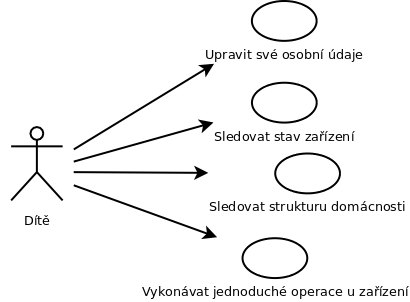
\includegraphics[width=0.4 \linewidth]{obrazky-figures/useCaseChild.png}
  \caption{Diagram užití pro roli \textbf{Dítě}}
  \label{figure:use_case_dite}
\end{figure}

\begin{figure}[hbt]
  \centering
  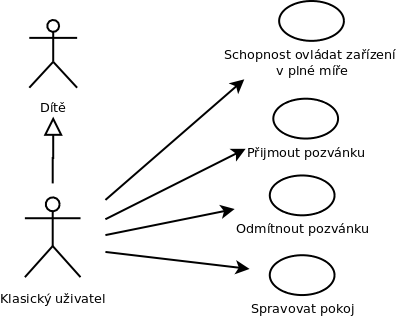
\includegraphics[width=0.4 \linewidth]{obrazky-figures/useCaseUser.png}
  \caption{Diagram užití pro roli \textbf{Klasický uživatel}}
  \label{figure:use_case_uzivatel}
\end{figure}

\begin{figure}[hbt]
  \centering
  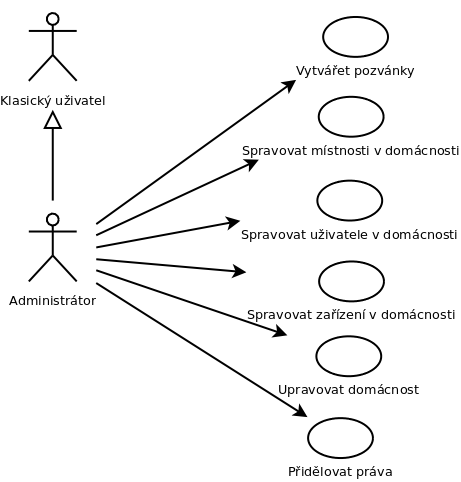
\includegraphics[width=0.4 \linewidth]{obrazky-figures/useCaseAdmin.png}
  \caption{Diagram užití pro roli \textbf{Administrátor}}
  \label{figure:use_case_admin}
\end{figure}

\newpage
\subsection*{Správa požadavků ze zařízení}
\label{backend:mqtt}

Důležitou součástí serverové části systému je správa požadavků ze zařízení asociovaných s~domácností.
Komunikace mezi zařízením a serverem probíhá pomocí protokolu \emph{MQTT}.
Pro každou domácnost existuje na serveru jedna instance \emph{MQTT} klienta.
U~každé domácnosti lze definovat pouze jeden \emph{MQTT Broker} a náležitá zařízení se připojují přímo k~němu.
Daná instance \emph{MQTT} klienta je přihlášená k~odběru celého provozu dané domácnosti.
Lze tak jednoduše odchytávat komunikaci mezi zařízeními v~domácnosti za účelem správy perzistentního obsahu u~zařízení.
Analýza provozu a komunikace u~zařízení slouží k~vytváření statistik posledních hodnot, které mohou být použity k~efektivnímu chodu domácnosti a její správě.
Lze tak efektivně řídit provoz elektricky náročných zařízení. Dále je možnost analyzovat data, která jsou dále zpracována pomocí většího výpočetního výkonu serveru, než u~daných zařízení a generovat tak příslušný výstup.

Pomocí protokolu \emph{MQTT} jsou spravovány i požadavky týkající se \emph{CRUD} operací daného zařízení.
Tyto operace jsou pouze přístupné zařízením a ne klientským aplikacím.
Zařízení je tak schopno zaslat požadavek na server, který spojí dané zařízení s~domácností, či připojení již existujícího zařízení a následně aktivovat dané zařízení pro přístup z~klientských aplikací.

\newpage
\section{Návrh databáze}
\label{navrh:databaze}

Návrh databáze úzce souvisí se serverovou částí systému. Server vytváří rozhraní, pomocí kterého lze vytvářet operace nad danou databází.
Server disponuje určitým \emph{ORM} frameworkem, který mapuje objektově orientovaný model do relační databáze a vývojař tak není nucen pracovat s~databází na nižší úrovni např. pomocí SQL jazyka.

Návrh databáze u~daného řešení chytré domácnosti je modelován pomocí \emph{ER diagramu}\footnote{\textbf{ER Diagram} - \textbf{E}ntity-\textbf{R}elationship \textbf{D}iagram (entitně vztahový diagram)}, kde jsou znázorněné entity\footnote{\textbf{Entita} - věc schopná samostatné existence} modelující tabulky databáze a jejich propojení.
Databáze je tak modelována pomocí modelovací jazyka s~názvem \emph{UML}.
Diagram obsahuje název entity, primární klíče, atributy entity a asociace tabulek s~určitou kardinalitou.

Mezi základní entity řešení chytré domácnosti patří:
\begin{itemize}
  \item \textbf{\emph{User}} - základní informace o~uživateli
  \item \textbf{\emph{Home}} - domácnost
  \item \textbf{\emph{Room}} - místnost/pokoj
  \item \textbf{\emph{Device}} - zařízení
  \item \textbf{\emph{Capability}} - schopnost zařízení
\end{itemize}

\subsection*{Entita \emph{User} - uživatel}
\label{databaze:user}
Entita \textbf{\emph{User}}(uživatel) obsahuje dva identifikátory. První z~nich je primární klíč celé entity a druhý identifikátor typu \emph{UUID}\footnote{\textbf{UUID} - \textbf{U}niversally \textbf{U}nique \textbf{I}dentifier (Univerzální unikátní identifikátor)} slouží k~identifikaci uživatele z~\emph{JWT} tokenu.
Tato tabulka je pouze pomocnou entitou v~udržování informací o~uživatelích. Primárním uložištěm informací je autentizační služba, která dále obsahuje i přístupová data.
Daná entita se využívá hlavně v~případě, kdy uživatel pro každou domácnost disponuje různými rolemi. Tato entita je dále využívána v~identifikaci uživatele v~pozvánkách do domácnosti.

\subsection*{Entita \emph{Home} - domácnost}
\label{databaze:home}
Nejdůležitějším celkem celé databáze je entita \textbf{\emph{Home}}, která obsahuje základní potřebné informace o~domácnosti.
Jako každá tabulka databáze musí mít přiřazený primární klíč s~jednoznačným identifikátorem dané entity.
Dále obsahuje prvek \emph{name}, který je typu \emph{String}(řetězec znaků) a je zde uložen název domácnosti.
Důležitým atributem entity je \emph{brokerURL}, což je URL \emph{MQTT} brokeru.
Domácnost může mít pouze jeden \emph{MQTT Broker}, tudíž stačí uložit jeden prvek s~typem \emph{String}.
Entita \emph{Home} dále obsahuje cizí klíč pro entitu \emph{MQTTClient}, kde kardinalita daného vztahu je 1:1 díky tomu, jak již bylo zmíněno, může být pouze jeden \emph{MQTT Broker} a \emph{MQTT Client} pro domácnost.
U~klienta se rozumí spíše klient, který spravuje a analyzuje zprávy z~komunikačního protokolu \emph{MQTT}.

\subsection*{Entita \emph{Room} - místnost}
\label{databaze:room}
Entita \emph{Home} je provázána s~entitou \textbf{\emph{Room}}.
Domácnost může obsahovat více místností, ale daná místnost může být zahrnuta pouze v~jedné domácnosti.
Dále je provázána s~entitou \emph{Device}(zařízení), kde představuje seznam zařízení, které nejsou zatím přiřazeny do určitého pokoje a jsou proto tzv. \emph{unassigned}(nepřiřazené).
Dále se k~entitě \emph{Home} vztahuje i entita \emph{HomeInvitation}(pozvánky do domácnosti), kde jsou ve vztahu 1:N kvůli tomu, že domácnost může obsahovat několik pozvánek, ale v~pozvánce může být zahrnuta pouze jedna domácnost.

Jako další provázána s~\emph{Home} entitou je entita \emph{User}, která je ve vztahu M:N.
Tento vztah představuje asociaci, kde domácnost může obsahovat více uživatelů a uživatelé mohou být obsažení ve více domácnostech.
Vytváří se tak jedinečná asociace v~celé databázi.
V~poslední řadě si uchovává množinu uživatelů, kteří tuto místnost vlastní a mají určitá vyhrazená práva k~místnosti.

\subsection*{Entita \emph{Device} - zařízení}
\label{databaze:device}
Podstatná entita systému je \textbf{\emph{Device}}, která obsahuje opět jednoznačný identifikátor, název zařízení a status, zda je zařízení aktivní.
Zařízení může být provázáno s~místností, nebo i s~domácností a proto tudíž obsahuje dva cizí klíče referující na \emph{Home} a \emph{Room}.
Pokud zařízení nemá přiřazeno žádnou místnost, automaticky je vložen do množiny, kterou spravuje entita \emph{Home} a obsahuje nepřiřazená zařízení.
Každé zařízení je lehce modifikovatelné a uživatel si může vytvořit své vlastní zařízení disponující určitými tzv.\emph{capabilities}(schopnostmi), jako je např. měření teploty, vlhkosti, ovládání světelných zařízení atd.

\subsection*{Entita \emph{Capability} - schopnost zařízení}
\label{databaze:capability}
Entita podřazená zařízení nese název \textbf{\emph{Capability}}. Tato entita obsahuje prvky, které jsou nejblíže samotnému HW zařízení.
Obsahuje identifikátor, název, příznak \emph{enabled}(zda je schopnost povolená), typ dané schopnosti a pin ke kterému je připojena komponenta zprostředkovávající schopnost připojena.
Kardinalita vztahu mezi entitou \emph{Device} a příslušnou entitou je v~poměru 1:N, kde zařízení může mít několik schopností a daná jednoznačná schopnost může být přiřazena jednomu zařízení.

\begin{figure}[hbt]
  \centering
  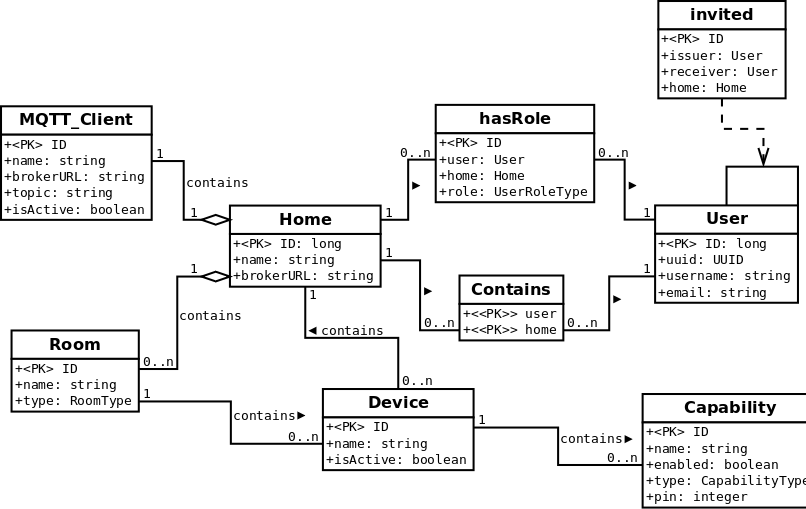
\includegraphics[width=0.9 \linewidth]{obrazky-figures/erdiagram.png}
  \caption{ER Diagram databáze}
  \label{figure:er_databaze}
\end{figure}

\newpage
\section{Návrh klientské aplikace}
\label{navrh:frontend}

Klientská aplikace slouží k~přímé interakci s~uživatelem a navrhovaným systémem.
Tato aplikace slouží ke správě domácností, místností, zařízení a všech dodatečných vlastností systému.
Pro přístup do aplikace je nutné být autentizován.
Zda uživatel autentizován není, je přesměrován na stránku autentizační služby, kde musí poskytnout své přihlašovací údaje, či jiným definovaným způsobem prokázat svoji identitu.
Po úspěšném přihlášení je uživatel automaticky přesměrován zpět do klientské aplikace, kde vidí obecný přehled.
Na této úvodní stránce vidí uživatel sebou definované oblíbené domácnosti, místnosti, zařízení, nebo dokonce jenom schopnosti zařízení(např. teplota určité místnosti, vlhkost atd.).
Dále je zde možnost vidět různé statistiky domácnosti, kde vedle historie změn prostředí různých místností může být i celková spotřeba domácnosti.

Klientská aplikace je ve stylu tzv. \emph{Dashboardu}, který se velice hodí pro různé informační systémy a systémy starající se o~správu.
Klientských aplikací může být větší množství a nemusí být přímo svázány s~aktuální.
Aktuální aplikace je v~tomto kontextu myšlena aplikace, která je vytvořena jako implicitní pro tuto bakalářskou práci (dále budeme uvažovat pouze tuto konkrétní).
Daná aplikace je vytvořena v~podobě webové aplikace, která je přístupná přes internetový prohlížeč.
Aplikace disponuje responzivním designem, tudíž je schopno v~upravené formě přistupovat k~aplikaci přes mobilní zařízení.

Jak již bylo řečeno, klientských aplikací může být několik, protože využívají \emph{API}, které definuje server a posílají požadavky na daný server.
Žádná hlubší aplikační svázanost s~touto určitou aplikací nemá vliv na chod systému.
Klientská aplikace také komunikuje se zařízeními pomocí protokolu \emph{MQTT}, ale tento protokol je ještě zabalený v~protokolu \emph{Websocket}(více info viz. \ref{mqtt:websockets}).

\begin{figure}[hbt]
  \centering
  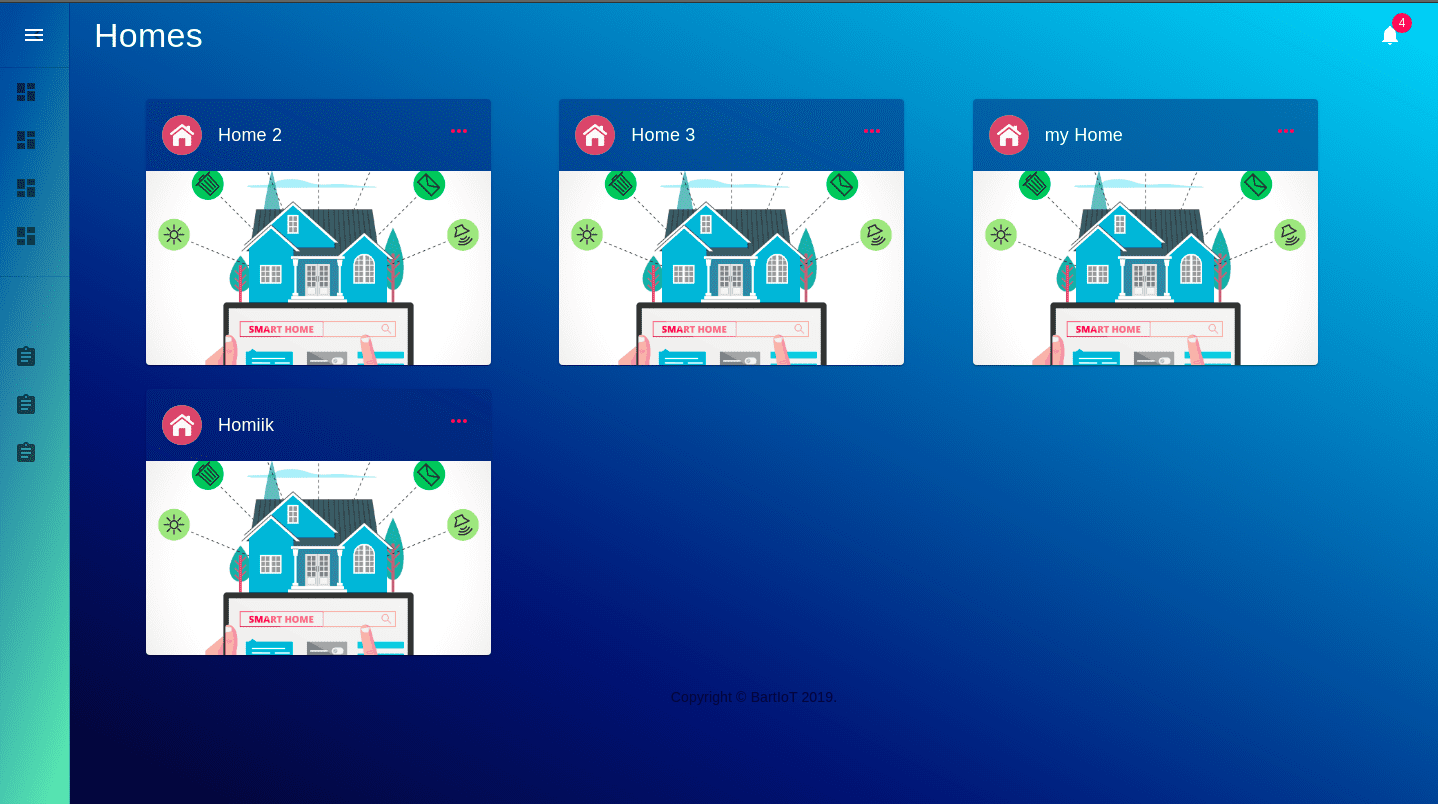
\includegraphics[width=0.9 \linewidth]{obrazky-figures/mockup.png}
  \caption{Vizuální návrh klientské aplikace}
  \label{figure:design}
\end{figure}

\newpage
\subsection*{Vzhled}
\label{frontend:vzhled}
Vizuální vzhled webové aplikace bude využívat tzv. \emph{tiles}(dlaždice), které představují různé komponenty aplikace(viz obrázek \ref{figure:design}).
Po levé straně aplikace(v desktop responzivní verzi) je postranní menu, které obsahuje navigační tlačítka, které uživatele přesměrují do jiných částí obsahu aplikace.
Důležitý prvek je položka s~názvem \emph{My Homes}, kde je po rozkliknutí uživatel přesměrován na stránku, která obsahuje všechny domácnosti, ve kterých je daný uživatel obsažen.
Domácnosti jsou také ve stylu dlaždic, kde ve spodní části obsahuje informaci o~roli uživatele, kterou má daný uživatel přiřazenou k~domácnosti.
V~právé spodní části je, pro většinu dlaždic obsažených v~aplikaci, tlačítko, které po rozkliknutí poskytne možnosti úpravy a správy dané dlaždice.

Po rozkliknutí dlaždice je uživatel přesměrován do dané domácnosti a opět ve stylu dlaždic jsou dostupné místnosti obsažené v~domácnosti.
Místnosti mají zase odlišnou nabídku možností, než jak to bylo u~domácností.
Uživatel v~daném prostředí má schopnost vytvořit si svojí místnost(zda má dostatečná práva).
Po dalším rozkliknutí dlaždice místnosti je uživatel přesměrován do dané místnosti, kde již vidí připojená zařízení a jejich \emph{capabilities}(schopnosti).
Schopnosti, mezi které se může řadit např. teplota místnosti, vlhkost, ovládání světel atd., jsou barevně odlišeny podle zařízení, do kterého patří. (např. schopnosti zařízení A~budou mít zelenou barvu a schopnosti zařízení B žlutou, atd.)

U~mobilních zařízení je postranní menu skryto a dlaždice jsou rozprostřeny souměrně na obrazovce podle velikosti displeje daného zařízení.
U~mobilních telefonů standardních rozměrů jsou tyto dlaždice vertikálně rozpoloženy v~jednom sloupci.
V~pravé horní části obrazovky je tzv. \emph{Hamburger menu}(tlačíko), které po rozkliknutí zobrazí postranní menu definované v~desktop responzivní verzi.

\subsection*{Programová část}
\label{frontend:program}
Programová část v~kontextu návrhu klientské aplikace se zabývá kompletní strukturou programu, či služeb, které probíhají na pozadí aplikace.
Aplikace se sestává z~jedné základní šablony, kde ostatní prvky, neboli komponenty, jsou dynamicky měněny.
Tudíž při přechodu na jinou záložku v~menu se nemusí vyrenderovat celá stránka, ale pouze změněné komponenty.
Klientská aplikace si udržuje stav, kterým právě uživatel disponuje.
Díky ukládání stavu do \emph{cache} prohlížeče uživatele je zamezeno několikanásobné posílání dotazů na server a plynulejší průchod aplikací.
Při každém požadavku na server a následném zpracování dat se změní i stav požadovaných informací uložených v~\emph{cache} prohlížeče.

Klientská aplikace je pomocí adaptéru na daný programovací jazyk připojena k~autentizační/autorizační službě se kterou inicializuje spojení a dále komunikuje.
Po autentizaci uživatele aplikace získá informace o~uživateli spravovaném autentizační službou pro další zpracování.
Zde se uloží atributy uživatele do objektu, který se následně uloží do autentizačního stavu.
Stav, který se stará o~autentizovaného uživatele obsahuje také \emph{access token}\footnote{\textbf{Access Token} - token pro přímý přístup ke zdroji informací; krátká životnost} a \emph{refresh token}\footnote{\textbf{Refresh Token} - token pro získání nového \emph{access} tokenu; dlouhá životnost}.
Autentizační služby nabízejí klientské adaptéry s~možností autonomního revalidování, nebo-li získání nového tokenu.
Programátor se tak nemusí starat o~vypršení časového limitu \emph{tokenu}.

Další vlastnost klientské aplikace je pracovat přímo se zařízeními i při výpadku serveru.
V~tomto případě však musí být zařízení už inicializovány na serveru a přidány do místnosti.
Poté lze přistupovat k~místnosti i bez aktivity serveru, kde se po rozkliknutí dané místnosti vytvoří instance \emph{MQTT klienta}, který dále přímo komunikuje přes \emph{MQTT broker} s~danými zařízeními.
Pro každou místnost se inicializuje jeden klient a pokud v~klientské aplikaci není rozkliknuta místnost spravující daná zařízení, klient inicializován není.
To ušetří mnoho instancí klientů, což je výhodou u~některých \emph{MQTT brokerů}, které povolují pouze dané množství klientů a nezahlcuje se tak ve velkém množství síť.

\section{Návrh HW zařízení}
\label{navrh:hardware}

Je to zařízení, které je schopno reagovat na vstupy, nebo akce a schopno generovat příslušný výstup.
Zařízení v~konceptu řešení této chytré domácnosti je soubor součástek spojených v~elektrickém obvodě lokalizovaných na \emph{DPS}\footnote{\textbf{DPS} - \textbf{D}eska \textbf{P}lošných \textbf{S}pojů}.
Hlavní komponentou celého zařízení je mikrokontrolér, který se stará o~všechny akce spojené s~daným zařízením.
Mikrokontrolér se dá považovat jako mozek daného zařízení.(více v~kapitole \ref{terminy:mcu})

Mikrokontrolér obsažený v~zařízení se stará i o~připojené vnější periférie, v~kontextu této práce o~tzv. \emph{capabilities}(schopnosti zařízení).
Schopnosti zařízení jsou připojené \emph{I/O} periférie k~\emph{MCU}.(např. teploměr, vlhkoměr, tranzistory ovládající světla,...)
HW zařízení jsou koncipována tak, aby byla jednoduše \emph{customizovatelná} pro zákazníkovy potřeby.
To znamená, že \emph{schopnosti zařízení} se dají lehce připojit, odpojit, či přidat jiný modul.
\newline

V~této bakalářské práci jsou braná v~potaz dva typy připojených zařízení:
\begin{itemize}
  \item \textbf{Dedikovaná energeticky úsporná}
  \item \textbf{Centrální pro místnost}
\end{itemize}

\subsection*{Dedikovaná energeticky úsporná}
\label{hardware:usporna}
První typ zařízení jsou dedikovaná energeticky úsporná zařízení, kde napájení pochází většinou z~nějakého akumulátoru a musí být maximálně energeticky nenáročná.
Tato zařízení by měla vydržet dlouhou dobu bez jakéhokoli zásahu a nabíjení akumulátoru.
K~tomuto typu zařízení lze pouze připojit malé množství \emph{I/O} periférií, neboli \emph{capabilities}.
Tato zařízení mají malou velikost a slouží pouze k~vykonávání dedikovaných operací bez značné míry \emph{customizace} za účelem efektivního přístupu ke zdrojům.
Mezi tyto schopnosti zařízení se řadí např. senzory, ovládání chytrých zásuvek(lze napájení získat jiným způsobem).

\subsection*{Centrální pro místnost}
\label{hardware:centralni}
Další typ zařízení jsou tzv. \emph{Centrální pro místnost}.
Tento typ zařízení je \emph{customizovatelný} ve velké míře a vyžaduje stabilní příjem energie, protože energetická náročnost těchto zařízení je vyšší oproti prvnímu typu a zařízení by vydržela pouze pár dní s~pomocí akumulátoru.
K~tomuto typu zařízení lze připojit větší množství \emph{I/O} periferií, neboli \emph{capabilities}.
Zařízení jsou dostupná v~místnostech a disponují základními schopnostmi, jako je měření teploty, vlhkosti, správa světelných aparátů atd.

\newpage
\subsection*{Komunikace a správa zařízení}
\label{hardware:komunikace}

Komunikace zařízení s~ostatními zařízeními, serverem, nebo s~brokerem probíhá pomocí protokolu \emph{MQTT}(více info viz \ref{terminy:mqtt}).
Před prvním použítím zařízení se musí zařízení inicializovat a získat potřebná data ze serveru.
Existují dva přístupy, jak se připojit k~serveru a aktivovat tak dané zařízení:
\begin{itemize}
  \item \textbf{Inicializace zařízení} - První použití zařízení
  \item \textbf{Opětovné připojení zařízení} - Opětovné použití zařízení
\end{itemize}

\subsubsection*{Inicializace zařízení}
Před prvním použitím, zařízení vytvoří \emph{WiFi AP}\footnote{\textbf{WiFi AP} - WiFi \textbf{A}ccess \textbf{P}oint (přístupový bod - samostatný přijímač/vysílač)}.
Uživatel se přihlásí k~danému AP pomocí hesla přiloženém k~zařízení. Zařízení má jednoznačný identifikátor, tudíž by neměla nastat kolize více zařízení.
Když je uživatel připojen, je vyžádán, aby otevřel určitou webovou stránku, která je zprostředkována zařízením - jedná se o~konfigurační stránku zařízení.
Po otevření webové stránky se uživateli zobrazí dostupné WiFi AP, uživatel vybere jeho domácí WiFi AP(připojení k~routeru, který je v~dané domácnosti).
Dále uživatel zadá webovou stránku, nebo IP adresu \emph{MQTT brokeru}, která je také přístupná s~dodaným softwarem, nebo zprostředkována administrátorem služeb.
Další základní parametr, který uživatel musí zadat, je identifikační číslo domácnosti.

Dále je možnost na dané stránce objevit výběr požadovaných schopností, které jsou dostupné namapované na daný port určitého mikrokontroléru.
Každý mikrokontrolér má většinou odlišné možnosti ve schopnostech poskytnout určitou funkcionalitu na port.
Konfigurace zařízení je tak dokončena a uložena do paměti flash daného mikrokontroléru.

Zařízení poté pošle \emph{MQTT} zprávu na určené téma, kterou odchytí server. Zpráva obsahuje název zařízení a dále pole \emph{capabilities}(schopnosti).
U~těchto schopností zařízení je přítomný typ schopnosti a pin, na kterém daná schopnost pracuje.
Zpráva v~poslední řadě obsahuje tzv. \emph{message ID}(identifikátor zprávy), který slouží k~identifikování odpovědi ze serveru.

Server zpracuje zprávu od zařízení a uloží zařízení a schopnosti do databáze.
Server zpět pošle zprávu typu \emph{CREATE} s~příslušnými identifikátory zařízení a schopností.
Obsahuje také stejný identifikátor zprávy.
Zařízení uloží do flash paměti dané identifikátory, je aktivováno a odebírá zprávy z~určitého \emph{topicu}.

\subsubsection*{Opětovné připojení zařízení}
Zařízení by v~tuto chvíli mělo být již inicializované.
Po zapnutí si zařízení přečte uložená data z~flash paměti.
Připojí se k~danému WiFi AP a pošle zprávu typu \emph{CONNECT} s~příslušnými identifikátory.
Server tak ověří, že zařízení má správně definovány příslušné identifikátory schopností a pošle zpět aktualizovaný seznam.
Zařízení se tímto úkonem aktivuje.

\newpage
\subsubsection*{Správa zařízení v~místnosti}
Další procedurou, kterou lze vykonat u~zařízení je přidání zařízení do domácnosti.
Zařízení musí být vždy obsaženo v~místnosti.
Když je přidáno do místnosti pomocí klientské aplikace, server po aktualizování záznamu o~zařízení v~databázi pošle zprávu o~přidání do místnosti.
Zařízení tak začne posílat hodnoty ze svých schopností na dané \emph{topicy}. Také začne přijímat zprávy z~daných topiců.
V~případě odebrání zařízení z~místnosti, je znovu zaslaná zpráva ze serveru a zařízení přestává posílat svá data ze schopností a čeká do té doby, než je zase přiřazeno do místnosti.
\newline

\subsubsection*{Smazání zařízení z~domácnosti}
Když je zařízení smazáno pomocí klientské aplikace, odebráno z~domácnosti, nebo smazaná domácnost, zařízení poté vymaže vše svá uložená data a přepne se do režimu, kdy musí být znovu inicializováno.
Uživatel tak musí znovu nastavit vše potřebné.

\newpage
\chapter{Použité technologie a komponenty}
\label{pouzite}

V~této kapitole jsou popsány technologie, služby a komponenty, které jsou využity pro implementaci návrhu řešení chytré domácnosti.
Použití všech těchto prvků bylo pečlivě zváženo a snaha využít nejlepší dostupné technologie a techniky, podle mého názoru, byla úspěšná.
Na obrázku \ref{figure:technologie_architektura} jsou znázorněny technologie, či služby, zakomponované v~architektuře systému.

V~podkapitole \ref{pouzite:backend} jsou technologie, které byly využity na implementaci \textbf{serverové části}, v~podkapitole \ref{pouzite:db} týkající se \textbf{databáze},
v~podkapitole \ref{pouzite:frontend} vše použité k~implementaci \textbf{klientské webové aplikace} a v~poslední podkapitole \ref{pouzite:hw} technologie a komponenty použité pro implementaci \textbf{hardwarové části} projektu.

\begin{figure}[hbt]
  \centering
  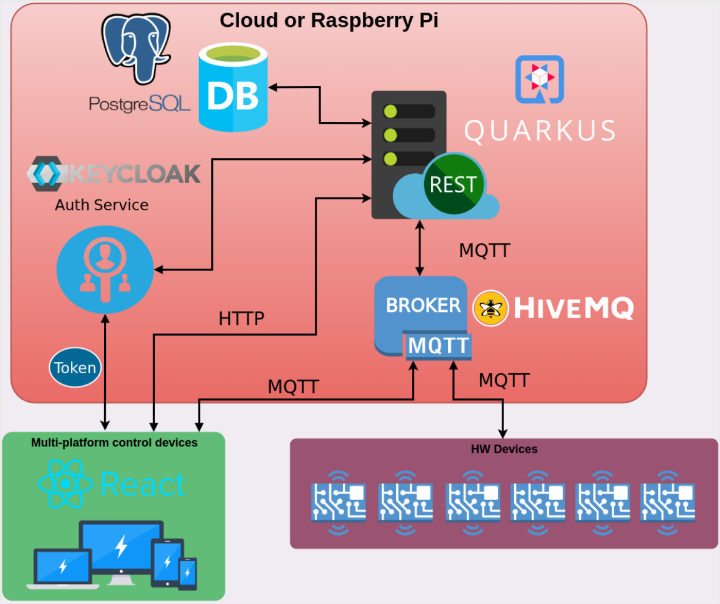
\includegraphics[width=0.9 \linewidth]{obrazky-figures/technologie.png}
  \caption{Použité služby v~architektuře}
  \label{figure:technologie_architektura}
\end{figure}

\newpage
\section{Serverová část}
\label{pouzite:backend}
Jak již bylo řečeno v~návrhu serverové části řešení chytré domácnosti, implementace serverové části je asi nejkomplikovanější z~celého vývoje řešení(pro více info viz \ref{navrh:backend}).
Pro účely vývoje serverové aplikace byl využit \emph{Java} framework zvaný \emph{Quarkus}(detailní popis \ref{pouzite:quarkus}).
Pro síťové služby spojené se serverovou částí byla využita sada nástroju s~označením \emph{Vert.x}(detailní popis \ref{pouzite:vertx}).

\subsection*{Quarkus}
\label{pouzite:quarkus}

\begin{figure}[!ht]
  \centering
  
\includegraphics[width=.45 \linewidth]{obrazky-figures/quarkus_logo.png}
  \caption{Quarkus logo}
  \label{figure:quarkus_logo}
\end{figure}

V~dnešní době, kdy žijeme v~době cloudových služeb, IoT a open-source projektů přichází do popředí kontejnery(\emph{containers}), mikroslužby(\emph{microservices}), reaktivní programování, cloud-native aplikace a spousty dalšího.
Díky těmto novým architekturám a nástrojům, přináší vývoj aplikací jiný rozměr a to speciálně větší produktivitu a výkonnost aplikací.
Programovací jazyk \emph{Java} už je na trhu přes 20 let a stálé zůstává mezi nejpopulárnějšími programovacími jazyky na světě.
V~informačních technologiích se však technologie a architektury mění velice rychle a je téměř nemožné využívat technologie přes 20 let bez větších změn. Aplikace v~kontejnerech by měly mít co nejmenší velikost, rychlý start při restartu a být škálovatelné.
To však v~případě dosavadních Java aplikací nebylo až tak možné. Framework \emph{Quarkus} by však měl vše změnit.

\textbf{Quarkus} je Kubernetes\footnote{\textbf{Kubernetes} - orchestrace kontejnerů na úrovni OS} Native Java framework, který nese označení \emph{Supersonic Subatomic Java} (nadzvuková subatomární Java).
Tento framework je přímo ušitý pro GraalVM\footnote{\textbf{GraalVM} - generuje nativní kód} a HotSpot(klasická JVM\footnote{\textbf{JVM} - \textbf{J}ava \textbf{V}irtual \textbf{M}achine}).
Je složen z~dostupných Java knihoven a standardů, které patří mezi ty nejlepší svého typu.
Vyznačuje se termínem zvaným \emph{Container First}, kde celý framework je založený na nasazení aplikací v~kontejnerech a dále v~cloudových službách.~\cite{quarkus:infoDev}

Na obrázku \ref{figure:quarkus_stats} je porovnání frameworku \emph{Quarkus} s~tradičním \emph{Cloud-Native} prvkem a dále porovnání vytvoření spustitelného souboru do nativního kódu pomocí \emph{GraalVM} a klasické využítí JVM pomocí \emph{OpenJDK}\footnote{\textbf{OpenJDK} - Open \textbf{J}ava \textbf{D}evelopment \textbf{K}it}.
Hodnoty jsou určeny pro klasickou \emph{REST}\footnote{\textbf{REST} - \textbf{RE}presentational \textbf{S}tate \textbf{T}ransfer (architektura rozhraní)} architekturu rozhraní a dále s~přidanými operacemi \emph{CRUD}\footnote{\textbf{CRUD} - \textbf{C}reate, \textbf{R}ead, \textbf{U}pdate, \textbf{D}elete (Vytvořit, Číst, Aktualizovat, Smazat)}.
První horizontální polovina obrázku se zabývá využítí paměti celého programu a závislostí.
Oproti tradičnímu \emph{Cloud-Native} prvku je program, vygenerovaný do nativního kódu, až 10x menší.
U~\emph{Cloud-Native} aplikací je to opravdu znatelný rozdíl.
V~druhé polovině je k~zahlédnutí nastartování celé aplikace a první odpověď ze serveru při požadavku.
Je zřejmé rapidní zvýšení rychlosti oproti klasickému tradičnímu \emph{Cloud-Native} prvku.
\emph{Quarkus} může být rychlejší více než 250x.~\cite{quarkus:website}

\begin{figure}[hbt]
  \centering
  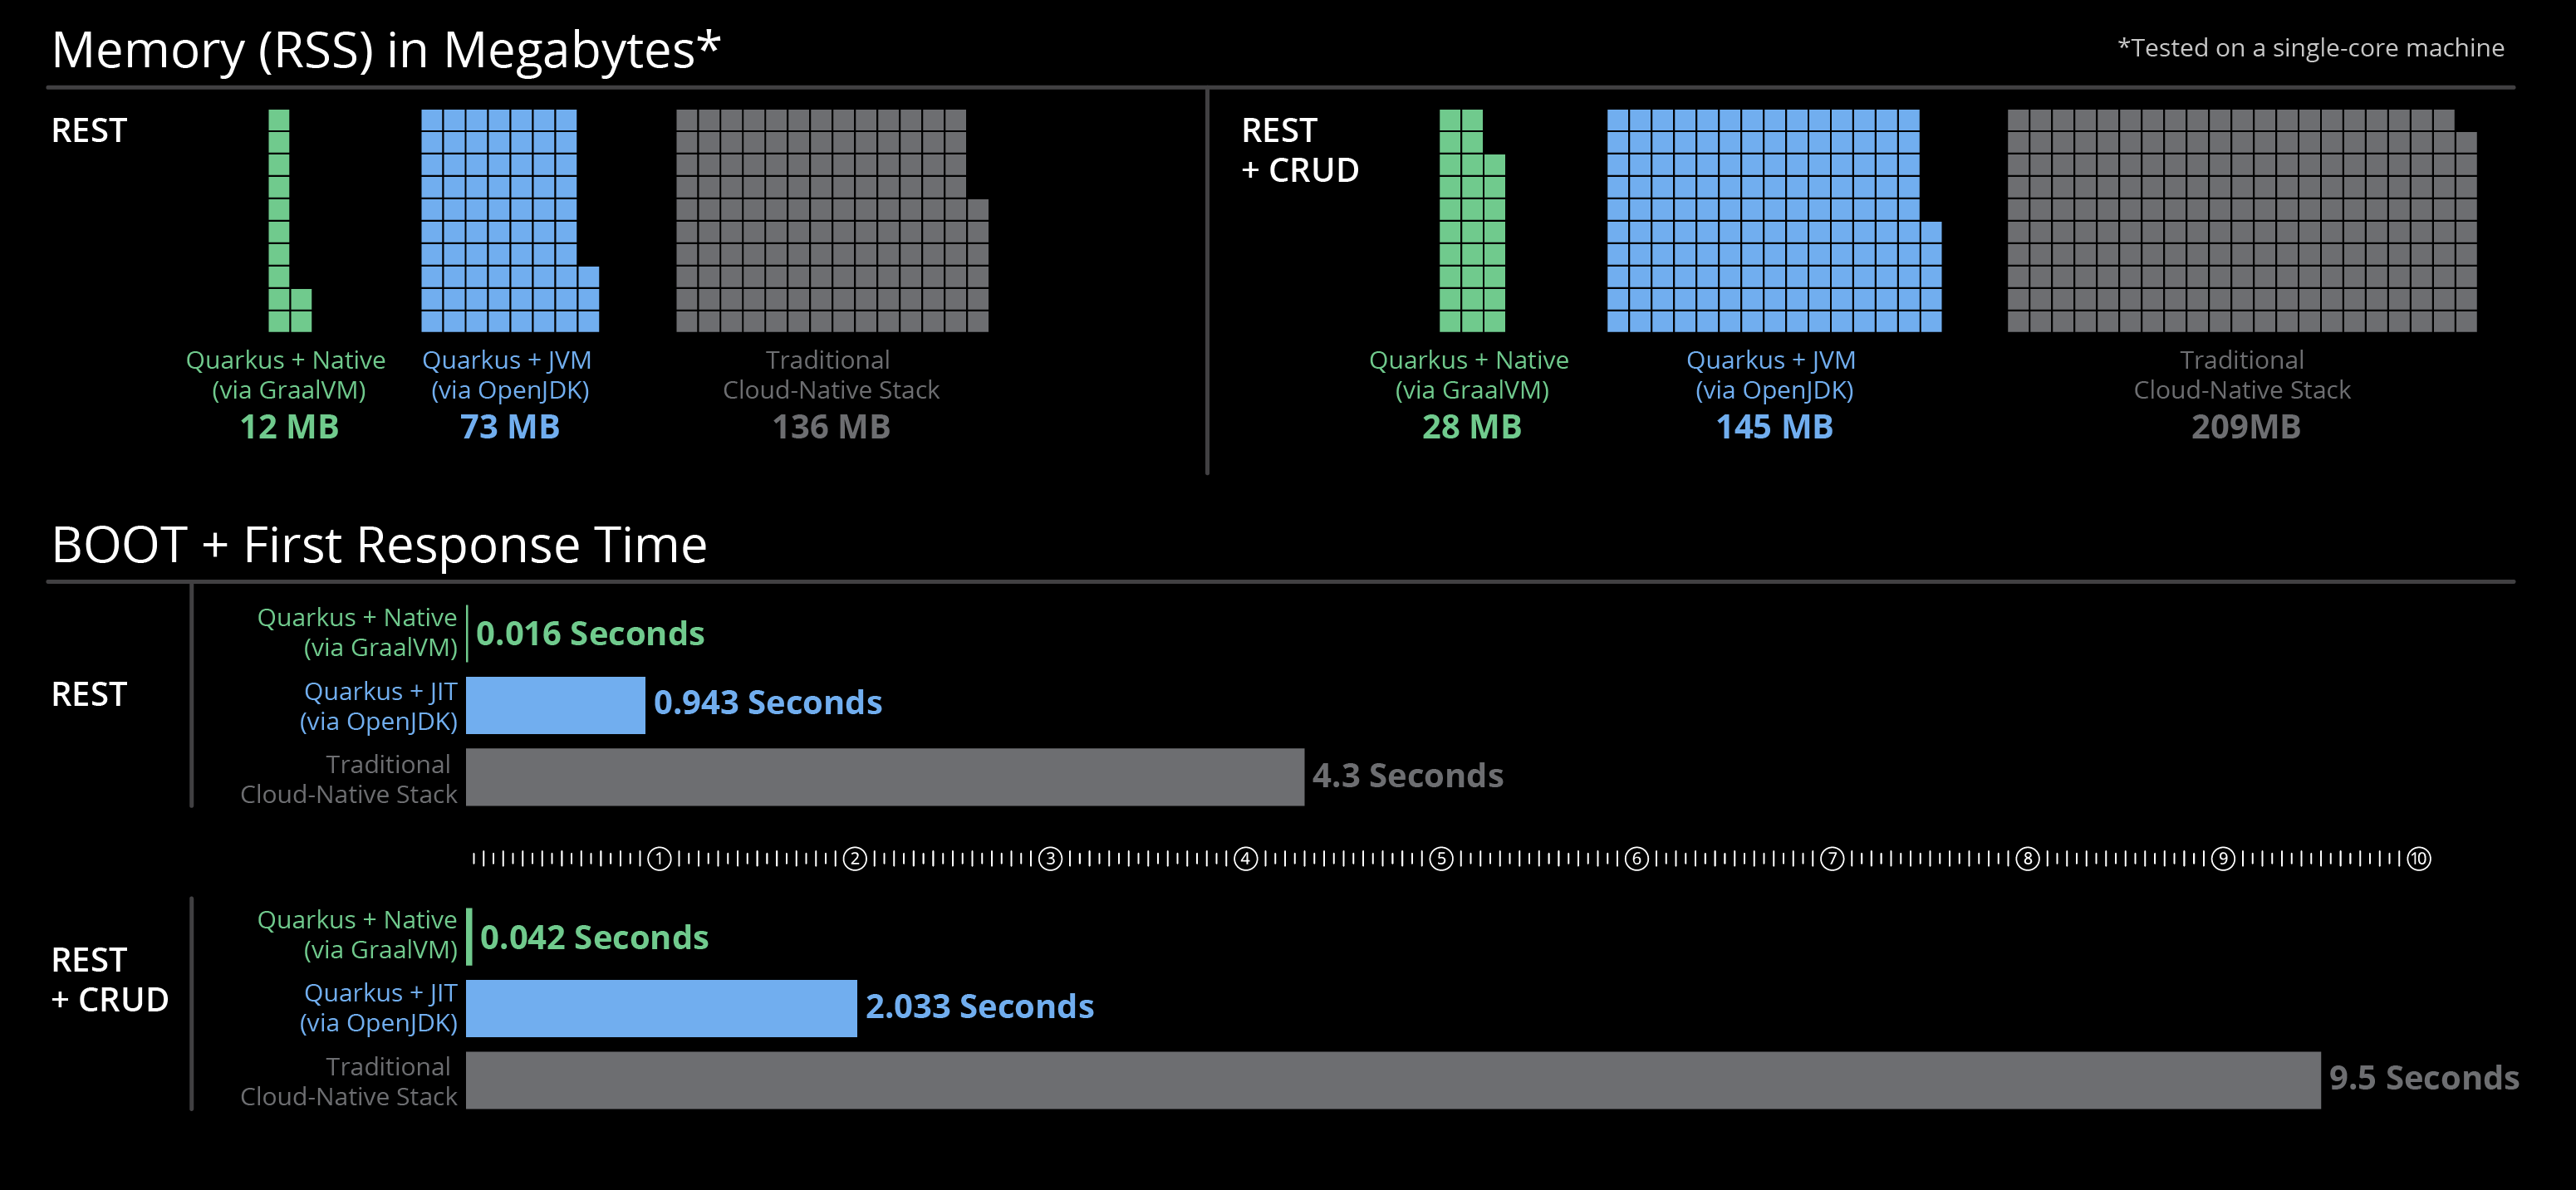
\includegraphics[width=1 \linewidth]{obrazky-figures/quarkus_stats.png}
  \caption{Porovnání frameworku Quarkus s~alternativami}
  \label{figure:quarkus_stats}
\end{figure}

\newpage
\subsection*{Vert.x}
\label{pouzite:vertx}
\begin{figure}[hbt]
  \centering
  
\includegraphics[width=.30 \linewidth]{obrazky-figures/vertx.png}
  \caption{Vert.x logo}
\end{figure}

\emph{Vert.x} je sada nástrojů pro vytvoření reaktivních aplikací, kde hlavní předností je malá velikost, nízké nároky na výpočetní prostředky a rozsáhlý ekosystém.
Samotný \emph{Quarkus} je založený na \emph{Vert.x} technologii a skoro všechny síťové featury v~technologii \emph{Quarkus} závisí na technologii \emph{Vert.x}.
Tato technologie přináší mnoho zajímavých vylepšení, jako jsou neblokující požadavky na server, jednoduchá souběžnost procesů (\emph{concurrency}), nebo například podpora několika programovacích jazyků.~\cite{wiki:vertx}

\section{Databázová část}
\label{pouzite:db}

\subsection*{Hibernate ORM}
\label{app_prostredi:hibernate}
\begin{figure}[hbt]
  \centering
  
\includegraphics[width=.2 \linewidth]{obrazky-figures/hibernate.png}
  \caption{Hibernate logo}
\end{figure}

\emph{Hibernate ORM} (dále pouze jako \emph{Hibernate}) je ORM\footnote{\textbf{ORM}- \textbf{O}bjektově \textbf{R}elační \textbf{M}apování} framework vyvíjen společností \emph{Red Hat}.
Poskytuje možnost mapování objektově orientovaného modelu do relační databáze.
Vývojář tak není zatížen vytvářením mezivrstvy, která konvertuje objekty a vytváří SQL dotazy na databázi.
Programátor tak může definovat tabulku databáze dvěma způsoby:
\begin{enumerate}
  \item Pomocí XML\footnote{\textbf{XML} - \textbf{E}xtension \textbf{M}arkup \textbf{L}anguage (značkovací jazyk)} mapovaní, kdy vývojář vytvoří XML soubor s~definovanými atributy tabulky a jejich omezeními.
  \item Vývojář pouze vytvoří POJO\footnote{\textbf{POJO} - \textbf{P}lain \textbf{O}ld \textbf{J}ava \textbf{O}bject (obyčejný \emph{Java} objekt)}, kde definuje tabulku v~relační databázi. Pomocí anotací se označí atributy třídy, které se namapují do tabulky databáze.
        Tímto způsobem lze vytvořit několik tabulek v~databázi a lze i pomocí anotací definovat asociaci mezi tabulkami a kardinalitu asociací.
\end{enumerate}
\emph{Hibernate} zprostředkovává rozhraní, které lze využít pro dotazy na databázi.
Vývojář může vytvořit vlastní metody, u~kterých lze definovat dotaz pomocí \emph{HQL}\footnote{\textbf{HQL} - \textbf{H}ibernate \textbf{Q}uery \textbf{L}anguage (dotazovací jazyk podobný \emph{SQL})} jazyka,
který je jednodušší a bližší samotným třídám (označovaným jako \emph{entity}).

\subsection*{PostgreSQL}
\label{pouzite:postgresql}
\begin{figure}[hbt]
  \centering
  
\includegraphics[width=.2 \linewidth]{obrazky-figures/postgresql-logo.png}
  \caption{\emph{PostgreSQL} logo}
\end{figure}

\emph{PostgreSQL} je objektově-relační, nejpokročilejší open-source databázový systém.
Byl vyvinut na Kalifornské univerzitě v~Berkeley.
Systém je vydáván pod \emph{MIT} licencí, tudíž ho lze svobodně distribuovat a měnit.
Byl hlavně navržen pro \emph{UNIX}ové systémy, ale později byl navržen tak, aby byl přenositelný na více platforem(např. \emph{Max OS X}, \emph{Solaris} a \emph{Windows}).
Vyžaduje pouze minimální úsilí na jeho údržbu díky jeho stabilitě.~\cite{postgres:tutorial}

Má za sebou více než dvacet let aktivního vývoje a má vynikající pověst pro svou spolehlivost a bezpečnost.
Výkonnostně nezaostává za srovnatelnými komerčními systémy a častokrát je i předčí.~\cite{postgres:wiki}
PostgreSQL byl vybrán pro účely implementace řešení této chytré domácnosti pro zmiňovanou stabilitu, spolehlivost a vysoký výkon.

\newpage
\section{Klientská aplikace}
\label{pouzite:frontend}

\subsection*{React}
\label{frontend:react}

\begin{figure}[hbt]
  \centering
  
\includegraphics[width=.3 \linewidth]{obrazky-figures/react.png}
  \caption{React logo}
\end{figure}

\emph{React} je JavaScript knihovna pro vytváření uživatelských rozhraní.
Tato knihovna je udržována společností \emph{Facebook} a komunitou developerů a společností.
React může být využit jako základ pro tvorbu single-page nebo mobilních aplikací, protože je optimální pro práci s~rychle se měnícími daty.
React se pouze zabývá renderováním dat do \emph{DOM}\footnote{\textbf{DOM} - \textbf{D}ocument \textbf{O}bject \textbf{M}odel (objektový model dokumentu)}.
V~aplikaci je dále použita další klíčová komponenta a to je \emph{React Router}, který se stará o~routování(směrování) v~aplikaci.
Dále je s~aplikací propojena i knihovna pro \emph{state management}\footnote{\textbf{State management} - (management stavu)} a to konkrétně \emph{Mob.x}.~\cite{react:info}

\subsection*{MobX}
\label{frontend:mobx}
\begin{figure}[hbt]
  \centering
  
\includegraphics[width=.1 \linewidth]{obrazky-figures/mobx.png}
  \caption{MobX logo}
\end{figure}

\emph{MobX} je knihovna, která tvoří \emph{state management} jednoduchý a škálovatelný pomocí \emph{TFRP}\footnote{\textbf{TFRP} - \textbf{T}ransparent \textbf{F}unctional \textbf{R}eactive \textbf{P}rogramming (transparentní použití funkcionálního reaktivního programování)}.
Knihovny \emph{React} a \emph{MobX} jsou velmi mocná kombinace, protože:
\begin{itemize}
  \item React renderuje stav aplikace takovým způsobem, že poskytuje mechanismus na překlad do stromů \emph{renderable}(schopných být renderovány) komponentů.
  \item MobX poskytuje mechanismus uložení a aktualizování stavu aplikace, který poté \emph{React} použije.
\end{itemize}

Jak \emph{React} tak i \emph{MobX} poskytují optimální a jedinečná řešení běžných problémů ve vývoji aplikací.
\emph{React} poskytuje mechanismus, který optimálně renderuje uživatelské rozhraní použitím virtuálního \emph{DOM}, který redukuje počet nákladných \emph{DOM} mutací.
\emph{MobX} poskytuje mechanismus, který optimálně synchronizuje stav aplikace s~\emph{React} komponenty pomocí
\emph{RVDSG}\footnote{\textbf{RVDSG} - \textbf{R}eactive \textbf{V}irtual \textbf{D}ependency \textbf{S}tate \textbf{G}raph (Reaktivní virtuální závislostní stavový graf)}, který je pouze aktualizovan v~případě, kdy je striktně potřeba.~\cite{mobx:info}

\newpage
\section{Hardwarová část}
\label{pouzite:hw}
V~této podkapitole jsou obsaženy moduly, které jsou využity v~daném řešení chytré domácnosti.
Konkrétní zařízení, která jsou v~kontextu této práce jsou sestaveny pomocí různých modulů obsahující mikročip \emph{ESP8266}(více v~podkapitole \emph{Moduly obsahující čip ESP8266}).
Pro nasazení služeb mimo cloud v~lokální síti je použit výkonný mini počítač s~označením \emph{Raspberry Pi 4B}(pro obecné info viz podkapitolu \emph{Minipočítač Raspberry Pi}).

\subsection*{Moduly obsahující čip ESP8266}
\label{terminy:esp8266}

\emph{ESP8266} je levný WiFi mikročip, který s~přidáním několika komponentů je schopen plnohodnotně plnit úlohu mikrokontroléru.
Tento mikročip je velice oblíbený v~oblasti chytrých zařízení díky své stabilitě, výkonnosti, velikosti, ceně a mnoho dalšího.~\cite{wiki:esp}
Na trhu existuje spousty modulů, které obsahují právě zmíněný mikročip a plní tak úlohu mikrokontroléru.

Mezi nejoblíbenější moduly, které obsahují tento mikročip jsou \emph{ESP-01}, který obsahuje pouze 2 GPIO\footnote{\textbf{GPIO} - \textbf{G}eneral \textbf{P}urpose \textbf{I}nput/\textbf{O}utput (univerzální vstupní/výstupní pin)} piny, poté větší \emph{Wemos D1 mini} a \emph{NodeMCU}.
Tento projekt chytré domácnosti je sestaven hlavně z~těchto modulů díky svým přednostem a využití.
Pro maximálně 2 jednotlivé I/O\footnote{\textbf{I/O} - \textbf{I}nput/\textbf{O}utput (vstup/výstup)} periferie připojené k~modulu je využit modul \emph{ESP-01}.
Pro komplexní využítí a připojení více periferií je použit modul \emph{Wemos D1 mini}.

\begin{figure}[hbt]
  \centering
  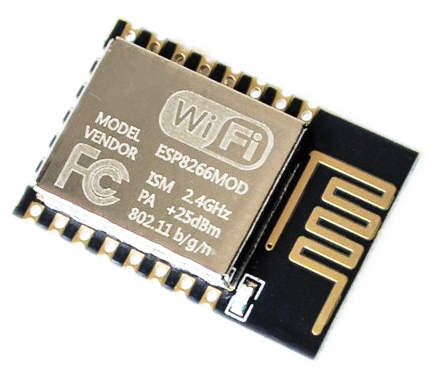
\includegraphics[width=.2 \linewidth]{obrazky-figures/esp_standalone.png}
  \caption{Samostatný ESP8266 čip}
  \label{figure:esp8266}
\end{figure}

\subsection*{Minipočítač Raspberry Pi}
\label{terminy:raspberry}

\emph{Raspberry Pi} je v~informatice označení pro jednodeskový počítač, který je se svým výkonem srovnatelný se slabším stolním počítačem.
Obsahuje video a audio výstupy,
ethernetový port, USB porty a výstup na dedikovaný monitor určený přímo pro \emph{Raspberry Pi}.
Tento malý počítač, rozměry podobný kreditní kartě, je využit v~této bakalářské práci na nasazení služeb, kdy uživatel nechce využívat cloudové služby.

Modelů \emph{Raspberry Pi} je na trhu více, kde se liší svým výkonem, velikostí, nebo kompatibilitou s~různými rozhraními.
Za účelem nasazení služeb v~chytré domácnosti lze využít i menšího sourozence z~rodiny počítačů \emph{Raspberry Pi} a to přesně \emph{Raspberry Pi W},
kde vytvořené, nebo poskytnuté služby jsou optimalizované pro běh na zařízeních s~menším výpočetním výkonem a operační pamětí.

\begin{figure}[ht]
  \centering
  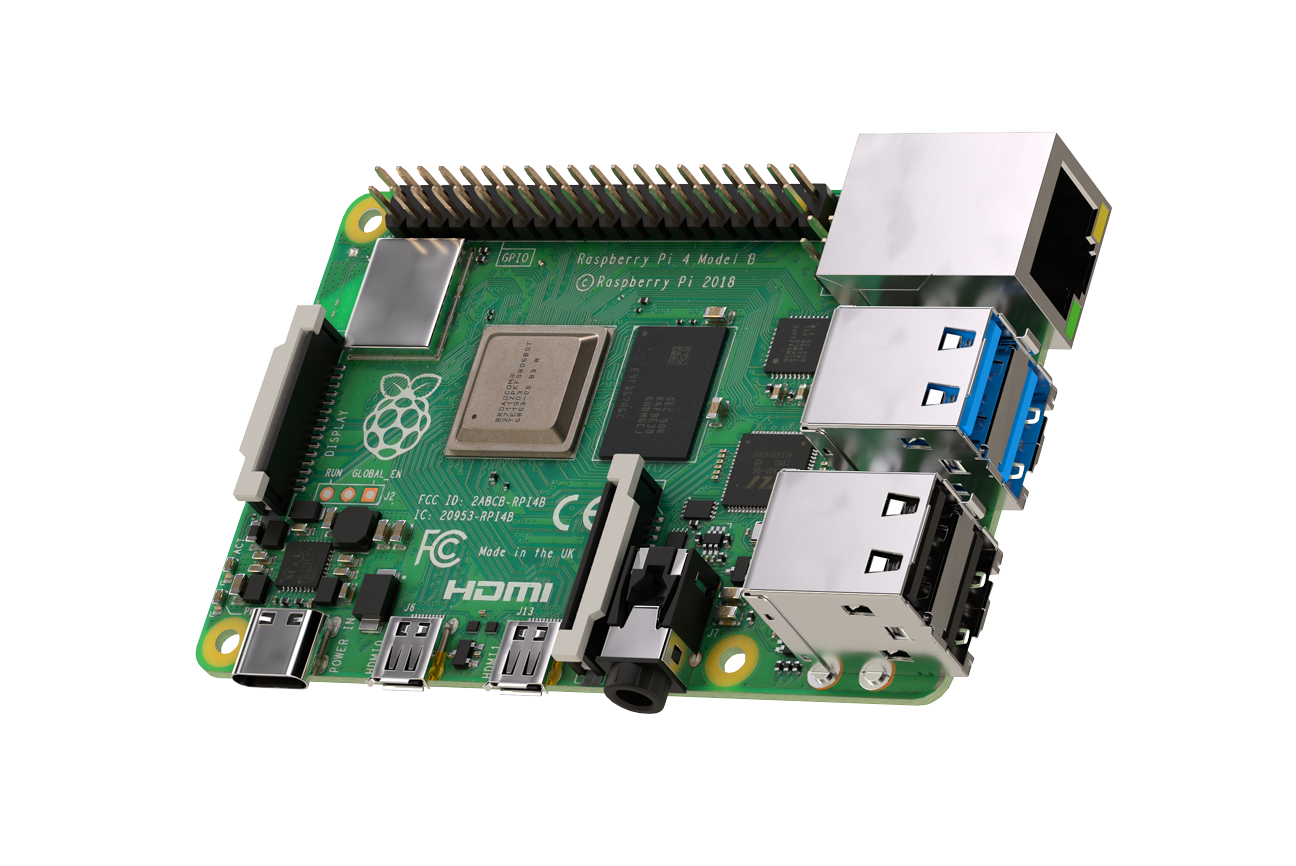
\includegraphics[width=.5 \linewidth]{obrazky-figures/raspberry.png}
  \caption{Raspberry Pi 4}
\end{figure}

\newpage
\section{Autentizační/autorizační služba}
\label{pouzite:auth}
Pro účely autentizace uživatelů v~klientské aplikaci a u~serveru je využita open-source služba s~názvem \emph{KeyCloak}.
Tento produkt využívám ve své práci pro autentizační služby a správu uživatelů.
Vývojář se tak nemusí starat o~perzistenci uživatelů a jejich správu.
O~vše se stará služba \emph{KeyCloak}.
\emph{KeyCloak} poměrně dobře znám, protože jsem jedním z~aktivních přispěvovatelů do projektu.

\subsection*{KeyCloak}
\label{terminy:keycloak}

\begin{figure}[hbt]
  \centering
  
\includegraphics[width=.25 \linewidth]{obrazky-figures/keycloak2.png}
  \caption{Keycloak logo}
\end{figure}

\textbf{KeyCloak} je open-source služba, která se stará o~autentizaci a autorizaci uživatelů a další předností je \emph{Identity and Access Management}(Management přístupu a identit),
kde administrátor může upravovat práva uživatelů, přidávat do skupin s~určitými právy apod.
Tato služba je podporována firmou \emph{Red Hat} a několik let už je v~popředí popularity služeb, které se starají o~bezpečnost webových aplikací. \emph{KeyCloak} disponuje rozsáhlou komunitou vývojářů, kteří jsou velice aktivní v~příspívání do daného komunitního produktu.
\emph{KeyCloak} obsahuje spousty nových vylepšení a je opravdu velice dobře škálovatelný(\emph{scalable}) a upravovatelný(\emph{customizable}).

Obsahuje spousty adaptérů pro klientské aplikace, tudíž nezáleží v~takové míře na programovacím jazyce.
Využívá standardní zabezpečovací protokoly, mezi které patří \emph{OIDC}, \emph{OAuth 2.0}\footnote{\textbf{OAuth 2.0} - autorizační protokol} a \emph{SAML 2.0}\footnote{\textbf{SAML 2.0} - \textbf{S}ecurity \textbf{A}ssertion \textbf{M}arkup \textbf{L}anguage (autentizační/autorizační protokol)}.
Lze dokonce využít i asociované autentizační a autorizační služby třetích stran pro udělení přístupu uživateli, registraci a mnoho dalšího.
Lze získat přístup i od tzv. \emph{social providers}(poskytovatelů identit ze sociálních sítí) jako jsou např. \emph{Facebook}, \emph{Google}, \emph{Twitter} apod.

Na obrázku \ref{figure:keycloak_flow} je popsán autentizační proces uživatele. V~prvním kroku uživatel žádá o~zdroj informací u~aplikace, která je asociována s~\emph{KeyCloak} aplikací (v~mém případě s~mojí \emph{backend} aplikací).
Aplikace pošle na službu \emph{KeyCloak} autentizační požadavek, služba se podívá, zda už je uživatel autentizován a když ano, pošle aplikaci odpověď o~úspěšném přihlášení a aplikace povolí uživateli přístup k~datům.

V~opačném případě je uživateli poskytnut seznam poskytovatelů služeb starající se o~identitu uživatelů.
Uživatel si může podle definovaného autentizačního toku (\emph{Authentication flow}) vybrat jakým způsobem se autentizuje. Když vše proběhne v~pořádku, \emph{KeyCloak} pošle odpověď aplikaci o~úspěšném přihlášení a uživatel dostane přístup k~datům.

\begin{figure}[hbt]
  \centering
  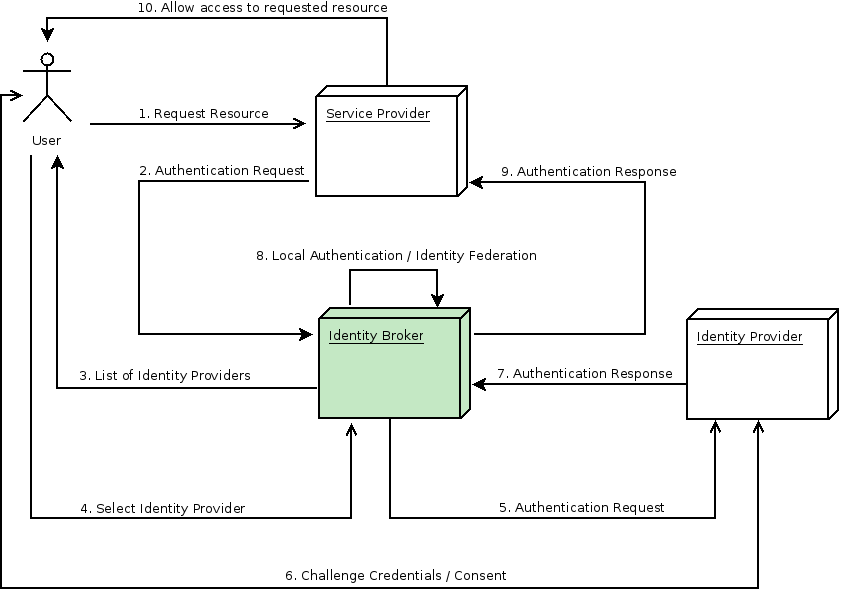
\includegraphics[width=.8 \linewidth]{obrazky-figures/keycloak_flow.png}
  \caption{Autentizační tok \emph{KeyCloak}}
  \label{figure:keycloak_flow}
\end{figure}

\section{Komunikace pomocí \emph{MQTT} protokolu}
\label{pouzite:mqtt}

V~této sekci lze nalézt knihovny a technologie určené pro bezproblémovou komunikaci pomocí \emph{MQTT} protokolu.
Nejdůležitější komponentou komunikace přes \emph{MQTT} protokol je \emph{MQTT Broker}(více info viz. \ref{terminy:mqtt}).
Instance pro poskytnutí brokeru byla využita služba \emph{HiveMQ}.

Každá část této aplikace(serverová část, klientská část, zařízení,...) komunikující přes daný protokol, musí disponovat knihovnou, která poskytuje rozhraní a implementaci standardních operací nad protokolem \emph{MQTT}(\emph{MQTT klient}).
Pro serverovou část a pro klientskou část to byla zvolena knihovna \emph{Eclipse Paho}.
Zvolená knihovna poskytuje knihovnu pro několik programovích jazyků a je velice rozšířená a oblíbená.
Pro HW zařízení byla zvolena knihovna \emph{PubSub} od autora se jménem \emph{Nick O'Leary} díky své jednoduchosti, spolehlivosti a výkonnosti.

\newpage
\subsection*{HiveMQ}
\label{pouzite:hivemq}

\emph{HiveMQ} je komunikační platforma navržená pro rychlý, efektivní, spolehlivý pohyb dat DO a Z~připojených \emph{IoT} zařízení.
Používá protokol MQTT pro okamžité obousměrné toky dat mezi zařízením a podnikovými systémy.
\emph{HiveMQ} je stvořen tak, aby dokázal čelit technickým výzvám, které organizace vyžadují u~vytváření nové \emph{IoT} aplikace.
\emph{HiveMQ} slouží jako \emph{MQTT broker} pro daný systém chytré domácnosti.
\newline
Prvky, které jsou nejdůležitější a \emph{HiveMQ} je řeší:
\begin{itemize}
  \item Vytvoření spolehlivé a škálovatelné \emph{IoT} aplikace.
  \item Rychlé dodání dat pro splnění očekávání koncových uživatelů.
  \item Nižší provozní náklady díky efektivnímu využití hardwarových, síťových a cloudových zdrojů.~\cite{hivemq:info}
\end{itemize}

\begin{figure}[hbt]
  \centering
  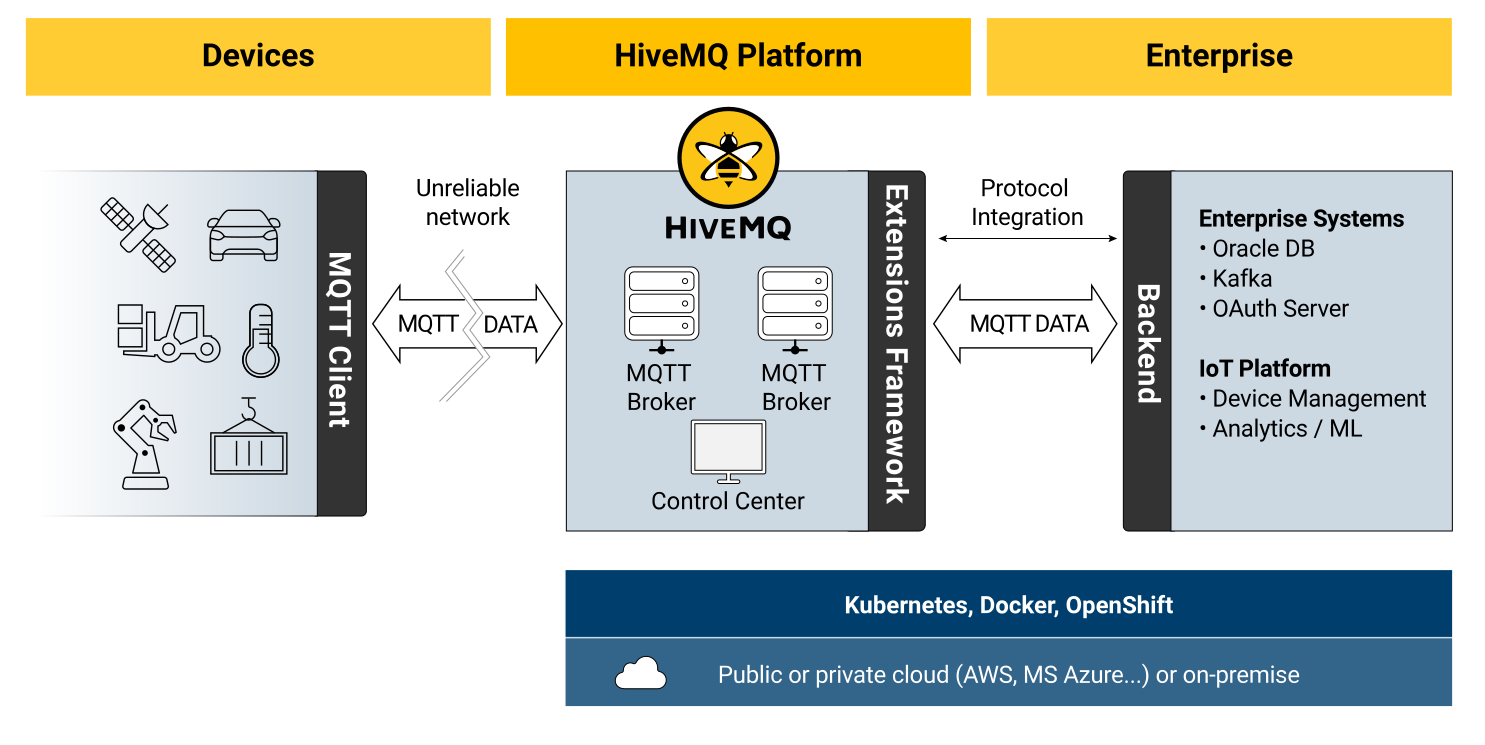
\includegraphics[width=1 \linewidth]{obrazky-figures/hivemq_arch.png}
  \caption{Enterprise architektura MQTT}
  \label{figure:hivemq_flow}
\end{figure}

\subsection*{\emph{Paho} knihovna}
\label{pouzite:paho}
\begin{figure}[hbt]
  \centering
  
\includegraphics[width=.2 \linewidth]{obrazky-figures/paho.png}
  \caption{Eclipse Paho logo}
  \label{figure:paho}
\end{figure}

\emph{Paho} projekt byl vytvořen pro poskytnutí škálovatelných open-source implementací otevřených a standardních komunikačních protokolů zaměřených na nové a
existující aplikace pro \emph{M2M}\footnote{\textbf{M2M} - Machine to Machine} a \emph{IoT} sítě.
\emph{Paho} odráží přirozené fyzické a náklady omezující možnosti připojení zařízení.
Cíle obsahují efektivní úroveň oddělení mezi zařízeními a aplikacemi, navrženou pro podporu rychlého růstu škálovatelného webového a podnikového middlewaru a aplikací.~\cite{paho:info}

\chapter{Implementace}
\label{implementace}
V~této kapitole je zahrnuto, jakým způsobem se dané řešení chytré domácnosti implementovalo.
Návrh řešení a použité technologie již byly popsány dříve (návrh v~kapitole \ref{navrh} a použité technologie v~kapitole \ref{pouzite}).
Návrh daného řešení byl směrodatný a obsahuje vše potřebné ke schopnosti implementovat dané řešení.
V~kapitole použitých technologií byly zavedeny také důvody výběru daných technologií a modulů.

Řešení chytré domácnosti je téma, které obsahuje různorodé prostředí obsažené v~komplexním systému.
Jedná se o~spojení serverové části, klientských aplikací, databáze a samotných hardwarových zařízení.
Návrh daného řešení je klíčový.
Postupem času, u~implementace daných prvků systému se požadavky, struktura a dokonce i architektura, měnili.
Hlavním důvodem bylo to, že při implementaci přicházely různé problémy, které se musely řešit.
Na způsob řešení implementačních problémů se vždy nějakým způsobem došlo a různé prvky aplikace jsou sestaveny po inspiraci z~různých větších produktů.
Tudíž, dané prvky systému by měly být architektonicky sestrojeny správným způsobem.

Implementace systému zahrnuje několik různých aspektů.
V~podkapitole \ref{impl:backend} je popsána implementace serverové části aplikace, v~podkapitole \ref{impl:frontend} implementace klientské aplikace.
Dále velice důležitá část implementace je perzistence dat v~systému a tudíž databáze. Zde je popsáno mapování, komunikace mezi serverem a databází (viz podkapitola \ref{impl:databaze}).
Poslední podkapitola \ref{impl:hw} se zabývá implementací daných HW zařízení komunikujících v~systému.

\section{Serverová část}
\label{impl:backend}
V~této podkapitole ja zahrnuta implementace serverové části aplikace, kde hlavním jádrem implementace je komunikace s~klientskými aplikacemi a HW zařízeními.
V~části komunikace s~danými prvky je nezbytné oddělit \emph{business} logiku od komunikačních prostředků.
V~aplikaci jsou zřízeny tzv. \emph{services}(služby), které udržují danou \emph{business logiku} ke které přistupují komunikační prostředky(\emph{REST controller, komunikace přes MQTT}).
Jak již bylo popsáno dříve v~návrhu, architektura serverové části aplikace dodržuje předpisy pro \emph{RESTful} aplikaci.
Tudíž se zde počítá s~bezstavostí požadavku na server.
V~podkapitolách serverové části budou zahrnuty nejdůležitější, nebo nejzajímavější implementační detaily implementace dané části.

\subsection*{Architektura}
\label{impl:backend:architektura}
Architektura serverové části systému(dále pouze jako \emph{aplikace}) je klíčová.
Aplikace je strukturována jako \emph{multi-module project}(projekt obsahující více modulů).
\newline
Tato struktura aplikace má spousty výhod:
\begin{itemize}
  \item \textbf{Separace logiky} - Oddělení \emph{business logiky} od dalších částí projektu. Moduly do sebe nezasahují.
  \item \textbf{Vysoká škálovatelnost} - Aplikace lze jednoduše rozšířit. Přídání dalšího modulu je jednoduché a není potřeba předělávat celou aplikaci. Platí i v~opačném případě při odebrání modulu z~projektu.
  \item \textbf{Udržovatelnost} - Vysoká míra udržovatelnosti aplikace a modulů.
  \item \textbf{Zachování \emph{API}} - \emph{API} je v~rámci celé aplikace většinou ve velké míře neměnné a mění se pouze implementace daného rozhraní s~rozdílnou logikou.
\end{itemize}

Jak je vidět z~výhod této struktury aplikace, je velice užitečná ve vývoji rozsáhlejší aplikace.
Dané aspekty jsou velice přínosné pro udržovatelnost a hlavně škálovatelnost aplikace, která je klíčová.
Moduly jsou vytvořeny pomocí buildovacího nástroje \emph{Maven}\footnote{\textbf{Maven} - nástroj na management projektu}.
U~většiny daných modulů se generuje samostatný \emph{JAR}\footnote{\textbf{JAR} - \textbf{J}ava \textbf{AR}chive} spustitelný soubor,
který je poté zakomponován s~dalšími do jednoho spustitelného souboru, který představuje celou serverovou aplikaci.
\newline
Základní moduly této aplikace jsou:
\begin{itemize}
  \item \textbf{API} - Definuje rozhraní pro přiložené moduly.
  \item \textbf{Authz} (\emph{Authorization} - Autorizace) - Stará se o~vlastní autorizaci celé aplikace.
  \item \textbf{Controller} ("Ovladač") - Řízení požadavků na server
  \item \textbf{Dist} (\emph{Distribution} - Distribuce systému) - Stará se o~kompozici modulů a vytváří tak komplexní aplikaci.
  \item \textbf{Persistence} (Perzistence dat) - Rodičovský modul modulů starající se o~perzistenci dat. Aktuálně pouze submodul \emph{JPA}.
  \item \textbf{Protocols} (Protokoly) - Komunikace aplikace pomocí dalších protokolů (\emph{MQTT}, \emph{WebSockets}).
  \item \textbf{Services} (Služby) - Udržuje \emph{business} logiku celé aplikace.
\end{itemize}

\newpage
\subsection*{Přijímání požadavků}
\label{impl:backend:request}
O~přijímání požadavku se stará implementace rozhraní \emph{JAX-RS}\footnote{\textbf{JAX-RS} - Java API for RESTful Web Services(rozhraní pro \emph{RESTful} služby)} a to přesněji \emph{RESTeasy}.
Tento framework používá anotace na usnadnění vývoje aplikací s~daným \emph{API}.
Přijímá a odesílá základní data pouze ve formátu \emph{JSON}.
Klient pošle požadavek na daný \emph{REST endpoint}, ke kterému je svázána nějaká operace(metoda), která se vykoná.
Každá třída implementující rozhraní pro přístup k~\emph{resources}(zdrojům) je vlastně \emph{Java Bean}\footnote{\textbf{Java Bean} - Java EE komponenta} se životností pouze po dobu vykonávání určitého požadavku (\emph{RequestScoped}), poté je destruována.

V~kódu níže je ukázka rozhraní, které vyobrazuje nastavení pro \emph{RESTeasy} framework.
Dané rozhraní se nachází v~modulu \emph{API} a implementace daného rozhraní v~modulu \emph{Controller}.
Jako první anotace použita na dané rozhraní je \annotation{@Path}, ve které se definuje cesta k~danému zdroji.
Dále následuje anotace \annotation{@Consumes} a \annotation{@Produces}, u~kterých je definovaná hodnota \emph{MediaType.APPLICATION\_JSON}.
Znamená to, že implementace daného rozhraní komzumuje a produkuje pouze informace ve formátu \emph{JSON}.

Anotace \annotation{@Transactional} značí, že požadavek na daný zdroj je brán transakčně, tudíž splňovat požadavky \emph{ACID}\footnote{\textbf{ACID} - \textbf{A}tomicity, \textbf{C}onsistency, \textbf{I}solation, \textbf{D}urability (Atomicita, Konzistence, Izolace a Trvanlivost)}.
Poslední \emph{class annotation}(anotace třídy) s~názvem \annotation{@Authenticated} značí, že uživatel musí být autentizován před vykonáním specifické operace.

Anotace \annotation{@GET} a \annotation{@POST} definují typy požadavku.
Lze použít i anotaci \annotation{@Path} na metody rozhraní, např. kdyby u~metody byla přidaná anotace \annotation{@Path} s~obsahem \emph{"/info"}, cesta k~danému zdroji
by musela mít podobu konkrétně \emph{"/homes/info"}.
Anotace \annotation{@Path} pracuje i s~parametry.
Uvažujme například \emph{URI} \emph{"/homes/3"}, které je možné namapovat pomocí anotace \annotation{@Path} s~parametry \emph{"/homes/\{id\}"}.

\begin{lstlisting}[style=JavaStyle, caption={Ukázka deklarování rozhraní pro správu domácností}]
  %%@Path%%("/homes")
  %%@Consumes%%(MediaType.APPLICATION_JSON)
  %%@Produces%%(MediaType.APPLICATION_JSON)
  $$@Transactional
  $$@Authenticated
  public interface !!HomesResource!! {

    $$@GET
    Response !!getAll()!!;

    $$@POST
    HomeModel !!createHome!!(String !!JSON!!);

    !!...!!
  }
\end{lstlisting}

\newpage
\subsection*{Předávání stavu při požadavku na server}
\label{impl:backend:state}

Jak již bylo v~předchozí kapitole určeno, framework na přijímání požadavků musí určit, jaké třídě, nebo metodě, směrovat požadavek.
To lze přidáním anotace \annotation{@Path}, v~které se definuje \emph{URI}\footnote{\textbf{URI} - \textbf{U}niform \textbf{R}esource \textbf{I}dentifier (jednotný identifikátor zdroje)}, které se musí shodovat s~cílem požadavku.
Každá třída reagující na požadavky od klientů má většinou definovanou cestu zdroje, o~který se stará.
V~úryvku kódu výše to bylo např. \emph{"/homes"}.
V~tomto úskalí však přichází problém.

\subsubsection*{Problém}
Systém řešení chytré domácnosti disponuje strukturou hierarchického rozpoložení zdrojů (např. \emph{homes -> rooms, rooms -> devices, devices -> capabilities,...}).
\emph{URI} každého zdroje obsahuje identifikátor každého prvku (např. \emph{"/homes/42}) díky kterému lze mapovat určitý jedinečný prvek.
Co když ale přijde situace, kdy potřebujeme dostat informace uložené ve schopnosti zařízení v~domácnosti s~identifikátorem 11, v~místnosti s~identifikátorem 22, zařízení s~identifikátorem 33 a schopnost s~identifikátorem 44.
\newline
Daná cesta ke zdroji vypadá konkrétně:
\begin{itemize}
  \item \emph{"/homes/11/rooms/22/devices/33/caps/44"}
\end{itemize}

Namapování takového zdroje pomocí anotace \annotation{@Path} by muselo vypadat takto:
\begin{itemize}
  \item \emph{@Path("/homes/\{homeID\}/rooms/\{roomID\}/devices/\{deviceID\}/caps/\{capID\}")}
\end{itemize}

Způsob zápisu je takřka nepoužitelný a nedovoluje škálovatelnost dané správy požadavků.
Může přijít situace, kdy budeme nuceni připojit k~cestě zdroje do zařízení další jiný zdroj.
Poté by jsme museli vytvořit další třídu, která tento ohromný zápis zpracuje.
Proto přichází řešení ve formě předávání stavu do různých komponent.

\subsubsection*{Řešení}
Vytvořil jsem \emph{Java Bean} komponentu s~názvem \emph{BartSession}, která má životnost také omezenou na vykonávání určitého požadavku.
Tato komponenta poskytuje uložení aktuálního stavu požadavku, distribuování \emph{services}(služeb) a informace o~autentizovaném uživateli.
Každá třída poskytující správu cílového zdroje z~požadavku (dále jako \emph{resource} třída) ve svém konstruktoru zahrnuje právě tuto komponentu.
Je tak zaručeno, že se stav dokáže předat do každé dané \emph{resource} třídy.

Při daném hierarchickém rozpoložení se lze z~jedné \emph{resource} třídy přesměrovat do další, z~dané třídy do další a tak dále, než se dorazí do požadované třídy obstarávající zdroj informací.
Každá \emph{resource} třída se stará pouze o~své vlastní zájmy a nepotřebuje vědět o~prostředí mimo ni.
Každá \emph{resource} třída disponuje různými metodami pro správu zdrojů.
V~úryvku kódu níže je vyobrazeno přesměrování požadavku do jiné \emph{resource} třídy s~poskytnutím změněného stavu.
Kód je pouze ilustrační; obsahuje pouze základní prvky potřebné pro ilustraci řešení.
\newpage
\begin{lstlisting}[style=JavaStyle, caption={Ukázka přesměrování požadavku}]
  // Rodicovska trida 'HomesResourceProvider'
  // implementujici rozhrani 'HomesResource'

  %%@Path%%("/homes")
  public class !!HomesResourceProvider!! implements !!HomesResource!! {
    BartSession !!session!!;
    !!...!!

    %%@Path%%("/{id}")
    public HomeResource !!forwardToSpecificHome!!(%%@PathParam%%("id") Long !!id!!){
      return new HomeResourceProvider(!!session!!.setActualHome(!!id!!));
    }
  }
\end{lstlisting}

\begin{lstlisting}[style=JavaStyle, caption={Ukázka zpracování požadavku z~přesměrované třídy}]
  // Podrazena trida 'HomeResourceProvider'
  // implementujici rozhrani 'HomeResource'

  public class !!HomeResourceProvider!! implements !!HomeResource!! {
    BartSession !!session!!;

    public !!HomeResourceProvider!!(BartSession !!session!!){
      this.!!session!! = !!session!!;
    }

    $$@GET
    public HomeModel !!getHome()!! {
      return !!session!!.getActualHome();
    }
    !!...!!
  }
\end{lstlisting}

\newpage
\section{Databázová část}
\label{impl:databaze}
Tato sekce pojednává o~propojení databázové části se serverem včetně způsobu mapování tabulek pomocí \emph{ORM} frameworku.
Uživatel posílající požadavky na server, po náležitých autentizačních/autorizačních operacích, dostane data právě ze zmiňované databáze.
Díky databázi jsou perzistentně uložená data, která slouží pro správu celé domácnosti.
Pro implementaci databázové části systému byla využita databáze \emph{PostgreSQL}(více info viz. \ref{pouzite:postgresql}).
Hlavní entitou databáze je samotná domácnost, kde je vytvořena asociace mezi dalšími tabulkami.

Jak již bylo řečeno v~návrhu, mezi databázovou vrstvou a serverovou vrstvou jsou objekty mapovány do relační databáze.
Ke schopnosti mapování tímto způsobem je zapotřebí \emph{ORM} framework, který jsem podle mého nejlepšího uvážení vybral konkrétně \emph{Hibernate ORM} (více info viz. \ref{app_prostredi:hibernate}).
U~\emph{Hibernate ORM} lze definovat entity pomocí anotací u~\emph{POJO}, nebo pomocí \emph{XML}.
Pro přehlednější, lépe škálovatelný přístup jsem vybral definování entit pomocí anotací.

\subsection*{Základní entita}

Na úryvku kódu níže je ilustrační příklad definování entity databáze u~třídy mapující domácnost.
Anotace \annotation{@Entity} slouží k~určení mapování-schopné třídy do relační databáze (povinné).
Další anotace \annotation{@Table} je nepovinná a slouží k~definování parametrů spojených s~tabulkou, např. definování jména tabulky.
Tato třída implementuje rozhraní \emph{HomeModel}, které deklaruje rozhraní pro operace nad domácností.
Pomocí rozhraní \emph{HomeModel} jsou entity dále, díky polymorfismu, v~aplikaci mapovány pouze jako dané rozhraní kvůli udržovatelnosti \emph{API}.

Každý atribut třídy je označen anotací \annotation{@Column}, která představuje sloupec tabulky.
U~této anotace lze např. definovat název sloupce, zda může být sloupec prázdný, atd.
Každá tabulka musí mít jednoznačný identifikátor a atribut plnící roli identifikátoru je označen anotací \annotation{@Id}.
Identifikátor může být také označen anotací \annotation{@GeneratedValue}, kdy se \emph{Hibernate} framework stará o~přiřazování jednoznačných identifikátorů sám.

\begin{lstlisting}[style=JavaStyle, caption={Ukázka definování entity}]
  $$@Entity
  %%@Table%%(name = "Homes")
  public class !!HomeEntity!! implements !!HomeModel!! {
  
      $$@Id
      $$@GeneratedValue
      %%@Column%%(name = "HOME_ID")
      Long !!id!!;
  
      %%@Column%%(nullable = false)
      String !!name!!;

      !!...!!
  }
\end{lstlisting}

\newpage
\subsection*{Asociace mezi entitami}
Jak to bývá zvykem u~relačních databází, tak v~tabulkách mohou existovat tzv. \emph{foreign keys} (cizí klíče), které se odkazují na identifikátor jiné tabulky.
Tím je vytvořena jakási asociace mezi tabulkami.
Existuje zde \emph{kardinalita}, která určuje četnost provázanosti tabulek.

Lze si to představit na příkladu z~daného řešení chytré domácnosti.
Tabulka představující domácnost je svázána s~tabulkou místností ve vztahu 1:N, což znamená, že domácnost může obsahovat několik místností, ale určitá místnost může být obsažena pouze v~jedné domácnosti.
\emph{ORM} framework \emph{Hibernate} nám umožňuje dokonce i namapovat dané asociace mezi entitami.
V~úryvku kódu níže je vyobrazen ilustrační kód pro definování asociace 1:N mezi domácností a místnostmi.

Entita vyznačující domácnost obsahuje množinu místností, které jsou připojeny k~domácnosti.
Anotace \annotation{@OneToMany} určuje asociaci ve vztahu 1:N (domácnost:místnosti), kde v~parametrech anotace je určena \emph{targetEntity}, ve které je definována cílová entita a
parametr \emph{mappedBy}, který představuje název atributu v~místnosi, pomocí kterého je domácnost mapována v~dané místnosti.

\begin{lstlisting}[style=JavaStyle, caption={Ukázka asociace 1:N (domácnost:místnosti)}]
  // Entita domacnost
  
  $$@Entity
  %%@Table%%(name = "Homes")
  public class !!HomeEntity!! implements !!HomeModel!! {
      !!...!!

      %%@OneToMany%%(targetEntity = !!RoomEntity!!.class, mappedBy = "home")
      Set<!!RoomModel!!> !!roomsSet!! = new HashSet<>();
  }
\end{lstlisting}

Entita vyznačující místnost obsahuje, jak již dříve bylo zmíněno, pouze referenci na jednu domácnost, ve které je daná místnost umístěna.
Anotace \annotation{@ManyToOne} určuje asociaci, inverzní vůči domácnosti, která definuje kardinalitu vztahů mezi entitami.
Anotace \annotation{@JoinColumn} slouží na propojení sloupců tabulek.

\begin{lstlisting}[style=JavaStyle,caption={Ukázka asociace 1:N (domácnost:místnosti)}]
  // Entita mistnost
  
  $$@Entity
  %%@Table%%(name = "Rooms")
  public class !!RoomEntity!! implements !!RoomModel!! {
    !!...!!

    $$@ManyToOne
    $$@JoinColumn
    HomeEntity !!home!!;
  }
\end{lstlisting}

\newpage
\section{Klientská část}
\label{impl:frontend}
Klientská aplikace se zabývá interakcí mezi uživatelem a systémem.
Tudíž je velmi důležitá v~kontextu řešení chytré domácnosti.
V~návrhu klientské aplikace je více informací o~struktuře klientské části (více info viz. \ref{navrh:frontend}).
Klientská aplikace byla implementována v~jazyce \emph{JavaScript} s~využítím knihovny \emph{React}(více info viz. \ref{frontend:react}).
Další důležitou součástí aplikace je udržovat stav aplikace o~který se stará nástroj \emph{MobX}(více info viz. \ref{frontend:mobx}).

Základem klientské aplikace je předpřipravená šablona ve stylu \emph{Dashboardu}, která je vydávána pod \emph{MIT} licencí, tudíž je volně šiřitelná.
Tato šablona je vytvořena pomocí knihovny \emph{Material UI}\footnote{\url{https://www.material-ui.com/}}. Autorem šablony je \emph{Creative Tim}\footnote{\url{https://www.creative-tim.com}}.
Ze šablony byla použita pouze kostra programu a některé jednoduché, dobře vypadající komponenty.

Aplikace je vytvořena z~komponent, které v~sobě obsahují další komponenty a obsažené komponenty obsahují další komponenty atd.
Jedná se o~kompozici komponent.
V~úryvku kódu níže je příklad vytvoření komponenty pomocí knihovny \emph{React}.

\begin{lstlisting}[style=JavaScriptStyle,caption={Ukázka definování komponenty}]
  export default function !!TestComponent!!(){
    const [state, setState] = React.useState(null);

    React.useEffect(() => {
      setState(42);
    }, []);
    
    return(
      %%<div>%%
        %%<p>%%This is test component%%</p>%%
        {state && %%<p>%%Number from state is: {state}%%</p>%%}
      %%</div>%%
    );
  }
\end{lstlisting}

Jak již bylo zmíněno, důležitou součástí klientské aplikace je i stav aplikace o~který se stará nástroj \emph{MobX}.
Pro aplikaci jsou vytvořeny tzv. \emph{stores}(úložiště), které slouží pro udržování stavu napříč aplikací.
\newline

Pro tento systém byly zatím vytvořeny základní úložiště a to:
\begin{itemize}
  \item \textbf{\emph{AuthStore}} - udržuje autentizační stav
  \item \textbf{\emph{HomeStore}} - udržuje stav domácnosti
  \item \textbf{\emph{RoomStore}} - udržuje stav místnosti
  \item \textbf{\emph{DeviceStore}} - udržuje stav zařízení
  \item \textbf{\emph{UserStore}} - udržuje stav uživatele
\end{itemize}

\newpage
V~úryvku kódu níže je příklad definování úložiště pomocí nástroje \emph{MobX}.
Nejzajímavější část celého \emph{store} je funkce \emph{decorate}.
Tato funkce definuje ve třídě atributy, které budou tzv. \emph{observable}(pozorovatelné).
Poté definuje \emph{action}(akce) metody,
které modifikují stav a \emph{computed}(vypočteno) getter, který vrací daný objekt/objekty.

\begin{lstlisting}[style=JavaScriptStyle,caption={Ukázka vytvoření \emph{store} pro domácnost}]
 export class !!HomeStore!!{
  _homes = new Map();

  setHomes = (homes) =>{
    this._homes = homes;
  }

  !!get!! homes() {
    return this._homes;
  }
 }

 %%decorate%%(!!HomeStore!!, {
    _homes: %%observable%%,
    setHomes: %%action%%,
    homes: %%computed%%
 });
\end{lstlisting}

\begin{figure}[hbt]
  \centering
  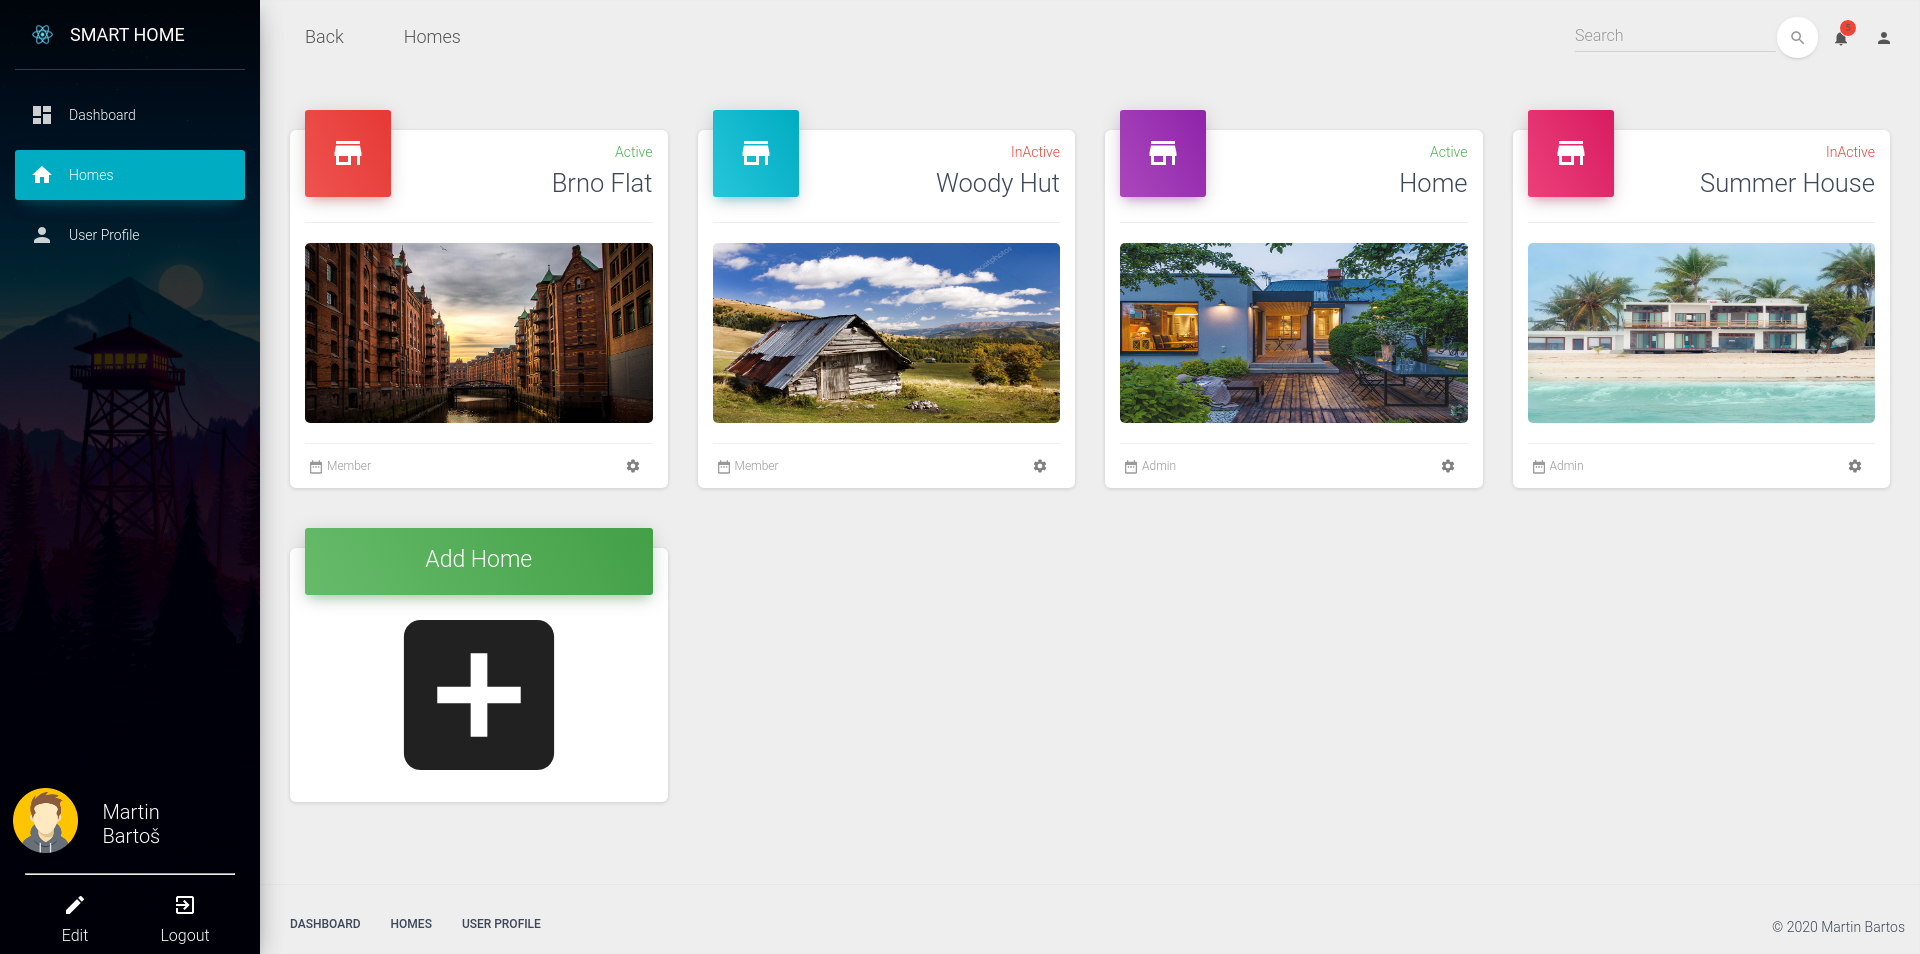
\includegraphics[width=1 \linewidth]{obrazky-figures/actualView.png}
  \caption{Aktuální vzhled aplikace}
  \label{figure:actual_app}
\end{figure}

\newpage
\section{HW část}
\label{impl:hw}
Hardwarová část systému chytré domácnosti je uzpůsobena pro komunikaci se serverovou částí a klientskou aplikací.
Jak již bylo popsáno v~návrhu, základem je mikrokontrolér, který slouží jako mozek celého zařízení(více info viz. \ref{terminy:mcu}).
Moduly, které jsou využity pro sestavení zařízení obsahují mikročip \emph{ESP8266}(více info viz. \ref{terminy:esp8266}).
V~návrhů řešení byly zařízení rozděleny do dvou kategorií.

Do první kategorie patří úsporná zařízení, která využívají modul \emph{ESP-01}, který disponuje pouze dvěma GPIO piny a hodí se pro různé samostatné senzory, či ovládání výstupních zařízeních.
Příkon tohoto modulu je opravdu nízký a podle mého názoru je tento modul velice vhodný pro dané úlohy.

Do druhé kategorie zařízení, které jsou centrální pro celou místnost, byly zvoleny moduly \emph{Wemos D1 mini}, které také využívají čip \emph{ESP8266}.
Tento modul využívá 11 GPIO pinů, tudíž lze připojit až 11 \emph{I/O} jednotek.

Program, který využívají tyto zařízení je naprogramován pomocí programovacího jazyka C++.
Kód je předpřipraven pracovat s~velkou řadou \emph{I/O} jednotek.
Je také velice dobře škálovatelný pro přidávání nových kompatibilních zařízení(pro více info viz. \ref{navrh:hardware}).
Jak již bylo zmíněno v~návrhu, tak pro zařízení byla zvolena knihovna, která umožňuje zařízením komunikovat přes \emph{MQTT} protokol s~názvem \emph{PubSub}.
Tuto knihovnu představil autor se jménem \emph{Nick O'Leary} a díky své jednoduchosti, spolehlivosti a výkonnosti jsem ji zařadil jako jádro komunikační části zařízení.

Díky knihovně \emph{WiFiManager}\footnote{\url{https://www.github.com/tzapu/WiFiManager}} od uživatele \emph{tzapu} bylo možné využít konfigurační webovou stránku při inicializaci zařízení.
Zařízení vytvoří svůj vlastní \emph{WiFi AP}, na který se uživatel připojí a poté je přesměrován na konfigurační stránku zprostředkovanou pomocí dané knihovny.

\begin{figure}[hbt]
  \minipage{0.5\textwidth}
  \centering
  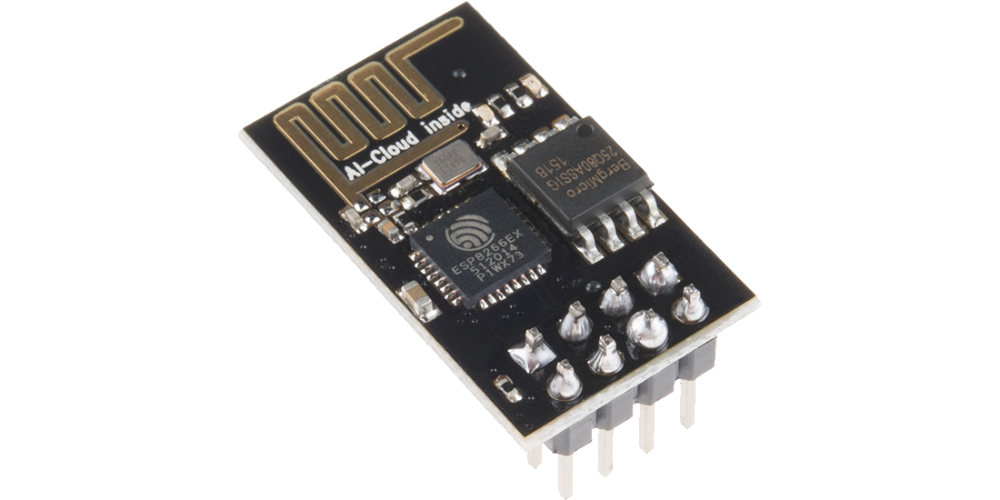
\includegraphics[width=.8\linewidth]{obrazky-figures/esp-01.png}
  \caption{Modul \emph{ESP-01}}
  \label{figure:esp01}
  \endminipage

  \hfill
  \minipage{0.5\textwidth}
  \centering
  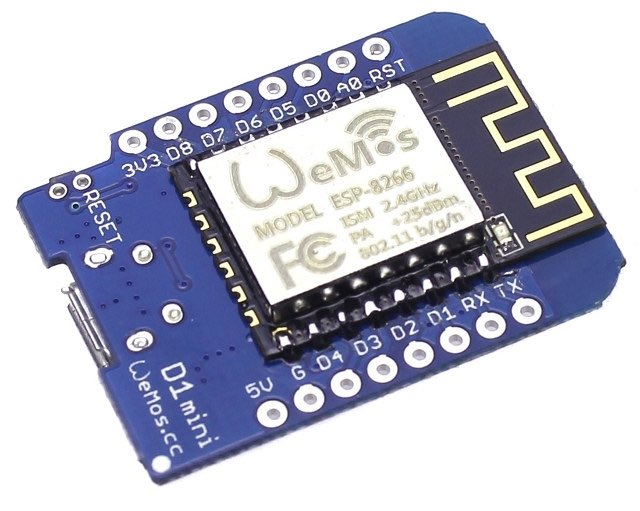
\includegraphics[width=.7\linewidth]{obrazky-figures/wemos.jpg}
  \caption{Modul Wemos D1 mini}
  \label{figure:wemos}
  \endminipage
\end{figure}

\begin{figure}[hbt]
  \centering
  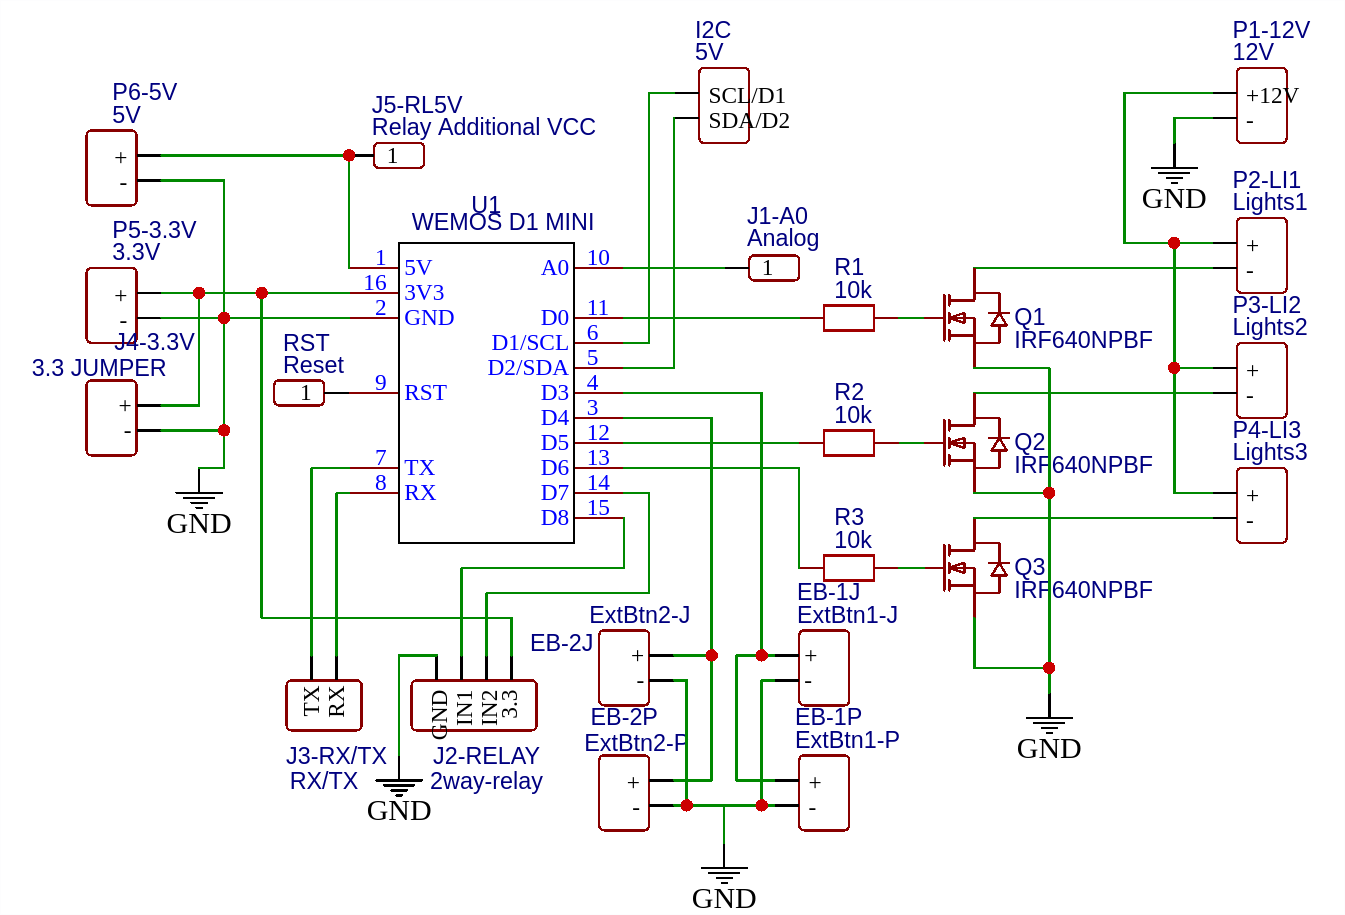
\includegraphics[width=1 \linewidth]{obrazky-figures/schematic.png}
  \caption{Návrh schématu centrálního zařízení}
  \label{figure:schema}
\end{figure}

\begin{figure}[hbt]
  \centering
  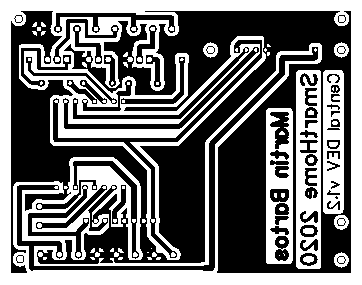
\includegraphics[width=0.6 \linewidth]{obrazky-figures/pcb.png}
  \caption{Návrh DPS pro centrální zařízení}
  \label{figure:schema}
\end{figure}

\chapter{Testování}
\label{testovani}
V~této kapitole je obsah zaměřen na testování celého systému řešení chytré domácnosti.
Důležitým faktorem daného řešení chytré domácnosti byla intuitivnost systému a to především uživatelského rozhraní.
Uživatel by pouze s~pomocí jednoduchého návodu měl být schopen zprovoznit svoji chytrou domácnost a vše správně nastavit.

V~kapitole \ref{testovani:UI} se testuje uživatelské rozhraní klientské aplikace a konfigurační stránky zařízení.
Dále v~kapitole \ref{testovani:praxe} je obsah směřován na využití systému v~praxi, kde byl systém nasazen v~mém vlastním pokoji.
Zde se otestovalo, jak moc stabilní daný systém je, zda splnil dané požadavky a jaká byla celková cena pořízení dané chytré domácnosti.
V~poslední \\ kapitole \ref{testovani:budouci} jsou zahrnuta vylepšení, která by mohla být do budoucna vykonána pro vytvoření lepšího řešení systému chytré domácnosti.

\section{Uživatelské rozhraní}
\label{testovani:UI}
Uživatelské rozhraní (dále jako \emph{UI}\footnote{\textbf{UI} - \textbf{U}ser \textbf{I}nterface (uživatelské rozhraní)}), plní velmi důležitou roli v~celém systému chytré domácnosti.
Díky \emph{UI} uživatel interaguje se systémem a je schopen spravovat celý systém.
Hlavním požadavkem \emph{UI} bylo vytvořit intuitivní klientskou webovou aplikaci a dále konfigurační webovou stránku pro zařízení.
Funkcionalita a daná intuitivnost \emph{UI} byla testována na členech rodiny a přítelkyni, kde skoro každý spadá do různé věkové kategorie, vše v~rozmezí 18-55 let.

Prvním krokem testování bylo vytvořit uživatelský účet, pomocí kterého se dále uživatel přihlašuje do systému.
Hned u~prvního kroku se došlo k~zajímavým výsledkům.
V~systému je zatím pouze podporována angličtina a testovaní uživatelé starší 50ti let s~tím měli poměrně značný problém díky své jazykové bariéře.
Mladší uživatele neměli téměř žádný problém, protože v~systému lze pracovat se základní angličtinou.
Zajímavým poznatkem byla u~registrace uživatele volba mezi vyplněním základních přihlašovacích údajů a využitím poskytovatelů identit ze sociálních sítí.
Většina mladých testovaných využila právě poskytnutí údajů ze sociálních sítí pro pohodlnější přístup a starší testovaní vyplňovali své údaje přímo.

Dalším krokem testování byla změna svých osobních a přihlašovacích údajů a následném odhlášení a přihlášení zpět do systému.
Zde nenastal žádný problém a uživatelé dokončili úspěšně tuto fázi bez jakýchkoli větších problémů a ztrátě orientace v~systému.
\newpage
Dále byli uživatele vyzvání k~vytvoření svého domu a místností uvnitř.
Daný úkol se jim také podařil vyřešit téměř ihned.
Každý uživatel dostal malou kartičku na které byly poskytnuty nezbytné adresy pro chod systému, např. \emph{URL} adresa \emph{MQTT Brokeru}, přístupové informace pro připojení k~\emph{WiFi} přístupovému bodu zařízení.
Uživatelé rychle pochopili princip dlaždic v~klientské aplikaci a správy daných dlaždic.
Většina dlaždic obsahuje tlačítko s~nastavením, kde jsou všechny dostupné operace, které lze provést s~danou dlaždicí.

Poté uživatel již může připojit své zařízení do domácnosti.
Uživatel připojil napájení pro zařízení díky \emph{USB} portu do počítače, či adaptéru.
Zařízení vytvořilo přístupový bod, na který se uživatelé připojili pomocí zmiňovaných přístupových informací.
Dále se otevřel webový prohlížeč, který zobrazil webovou stránku s~konfigurací zařízení.
Uživatelské rozhraní je jednoduché a velice intuitivní a uživatelé neměli problém s~poskytnutím informací pro zařízení.
Vybrali ze seznamu svůj \emph{WiFi} přístupový bod a zadali heslo.
Dále zde museli také zadat adresu \emph{MQTT Brokeru} a identifikační číslo domácnosti, které našli v~klientské aplikaci také jednoduše.
Zařízení si uchovalo informace pro pozdější připojení zařízení.

Uživatelé se vrátili do klientské aplikace.
Zde nastal problém s~tím, že někteří uživatelé nevěděli, jak postupovat dále.
V~této části musí uživatel v~nastavení místnosti zvolit volbu pro přidání zařízení do místnosti.
Je nutné přidat element, který pomůže uživatelům se zorientovat v~přidání zařízení.
Poté vybrali, po malé pomoci, dané zařízení a přidali do místnosti.
Po rozkliknutí se objevily schopnosti zařízení, se kterými již pracovali úspěšně.

\section{Kompletní systém v~praxi}
\label{testovani:praxe}
Jak již bylo popsáno v~implementaci řešení chytré domácnosti, snažil jsem se vytvořit i vlastní \emph{HW} zařízení osazené součástkami, plnící funkci schopností daného zařízení.
Zařízení bylo zkonstruováno jako centrální zařízení pro místnost obsahující mikrokontrolér \emph{Wemos D1 mini}, dva unipolární tranzistory MOSFET na ovládání LED světel, teploměr, vlhkoměr a nakonec dvě relé na spínání větších proudů a zařízení na 230V (např. větrák, lampa, atd.).
Dále je k~zařízení možno připojit další 3 různá zařízení na digitální vstupy mikrokontroléru.
Systém byl implementován v~mém pokoji, který obsahuje hlavní světla a podsvětlení nábytku složená z~bílých LED pásku.
Tato světla byla propojena s~daným zařízením a lze je ovládat pomocí systému.
Pro tato osvětlení byl použit zdroj ATX ze starého počítače, který slouží pro napájení samotných světel, ale také poskytuje 5V a 3.3V pro napájení samotného zařízení, tudíž není nutnost využívat více zdrojů energie.

Dále v~místnosti je využit modul \emph{ESP-01}, který je součástí relé modulu a má tak dedikovanou funkci správy relé.
Daný modul je využit pro spínání větráku v~místnosti.
V~pokoji je zahrnut ještě jeden stejný modul pro spínání lampy.
Zařízení v~pokoji lze snadno ovládat a existují pouze mírné nedostatky z~pohledu zmiňovaného uživatelského rozhraní, kdy si uživatel zatím nemůže měnit rozpoložení schopností zařízení na obrazovce a jejich velikost.
Pro nasazení služeb je zde využit minipočítač \emph{Raspberry Pi 4B}, který je připojen k~domácí \emph{WiFi} a tudíž mohou být zařízení připojena všude v~dosahu signálu \emph{WiFi} přístupového bodu.
Daný minipočítač je velmi výkonný a pro dosavadní implementaci systému by mohl být využit slabší modul.
Zařízení v~domácnosti se ale mohou rychle rozrůst a minipočítač bude velice vhodný pro danou funkcionalitu systému.
\newpage
Po stránce finančních nákladů implementace systému v~dané místnosti byl nejdražší minipočítač \emph{Raspberry Pi 4B}, který stál přibližně 1500kč.
U~centrálního zařízení pro místnost byl nejdražší mikrokontrolér \emph{Wemos}, který vyšel přibližně na 30kč, relé na 20kč, deska a další součástky asi na dalších 40kč.
Celková cena pro centrální zařízení se pohybuje okolo 90kč.
U~relé modulu s~mikrokontrolérem \emph{ESP-01} se cena pořízení pohybovala okolo 40kč.
Součástky byly zaslány přímo z~Číny a při koupi stejných součástek v~České republice by tato cena byla minimálně 4x vyšší.

\section{Návrh budoucích vylepšení}
\label{testovani:budouci}
Každý systém má samozřejmě určité nedostatky, které by pro lepší efektivitu mohly být vyřešeny a vylepšeny.
Během testování se přišlo na sadu zajímavých vylepšení a dá se říct, že systém funguje podle očekávání a dané vylepšení jsou pouze minoritní.
Tuto kapitolu jsem rozdělil na pár dalších podkapitol, které obsahují návrhy na vylepšení do budoucna.

V~podkapitole \ref{testovani:navrh:server} jsou vypsány mírné nedostatky u~serverové části systému a vylepšení, která by mohla vést k~lepší správě systému.
Podkapitola \ref{testovani:navrh:frontend} se zabývá klientskou aplikací, skrze níž uživatel interaguje se systémem.
V~další podkapitole \ref{testovani:navrh:hw} jsou popsány nedostatky u~HW zařízení a v~kapitole \ref{testovani:navrh:ostatní} ostatní vylepšení pro systém.

\subsection*{Serverová část}
\label{testovani:navrh:server}
U~serverové části systému je mírným nedostatkem management \emph{MQTT klienta}, který se stará o~správu zařízení a ukládání dat ze zařízení do databáze.
Daný klient obstarává každou zprávu ze zařízení pro domácnost a správa klienta je občas celkem náročná a tím pádem se jedná o~větší vytížení serveru.
Pro vylepšení dané záležitosti bych navrhoval použití některé existující streamovací služby, která se bude starat o~zprávy ze zařízení a bude lepší management zpráv.
Zatím nejlepším adeptem na danou fukncionalitu je podle mého názoru služba \emph{Apache Kafka}\footnote{\url{https://www.kafka.apache.org/}}.
Daná služba pracuje velmi dobře s~protokolem \emph{MQTT} a je schopna plnohodnotně nahradit i \emph{MQTT Broker} pomocí \emph{MQTT Proxy}.
Myslím si, že daná služba má velikou budoucnost ve streamovacích službách.

Dalším navrhovaným vylepšením je využití plné funkcionality služby \emph{Vert.x} zmíněné v~implementaci řešení.
Společně se službou \emph{RestEasy} se stará o~přijímání požadavků od klientů.
Vylepšení by spočívalo ve využití neblokujících operací, reaktivního programování a dalšího.
Dané změny by zvýšili několikanásobně výkon správy požadavků uživatelů.

\subsection*{Klientská aplikace}
\label{testovani:navrh:frontend}
U~klientské aplikace také existuje pár nedostatků.
Jde především o~některé minoritní záležitosti, jako např. přidání tlačítka na přiřazení zařízení k~domácnosti, změna fotografií u~uživatelského účtu, domácností a místností.
Dalším prvkem, který bych do budoucna rád vyřešil je seřazování dlaždic podle oblíbenosti uživatele, úprava velikosti dlaždic a funkce \emph{Drag and Drop}, která umožňuje uživateli uchopit dlaždici a umístit ji na požadované místo.

Dalším vylepšením pro klientskou aplikaci je podpora různých notifikací.
Uživatel by si tak mohl nadefinovat akci, která by vedla k~provedení jakési akce a následnému zaslání notifikace o~stavu operace.
Potřeba budou i komponenty pro časovače, které budou reagovat na určitou časovou událost a vykonávat definované operace.
V~poslední řadě se jedná o~zobrazení statistik dat ze zařízení pomocí určitých grafů apod.

\subsection*{HW zařízení}
\label{testovani:navrh:hw}
U~HW zařízení hraje velkou roli i konstrukční řešení.
Výroba samotného zařízení v~domácím prostředí má své nedostatky.
Především jde o~techniku výroby \emph{DPS}, kde v~omezených podmínkách byla vytvořena pomocí toneru z~tiskárny a dané nažehlovací techniky.
Tato technika není příliš přesná a vyžaduje širší vodivé cesty, což vede na větší velikost desky.
Testovací verze desky byla pouze jednostranná a zvětšila se zase o~větší kus.
Do budoucna bych si rád nechal vyrábět desky od dedikovaných poskytovatelů daných služeb pomocí \emph{SMD} technologie, kde součástky jsou velice malé, desky oboustranné a podpora rozsáhlejších možností návrhu.
Deska vyrobena pomocí \emph{SMD} technologie oproti klasickému způsobu může být i 4x menší.

Dále při testování zařízení se došlo k~závěru, že správa zařízení pomocí protokolu \emph{MQTT} není velice vhodná.
Zařízení totiž pro připojení k~serveru posílá celkem objemná data a zadaný protokol není přímo určený k~těmto záležitostem.
Je zde využita technika identifikátoru zprávy, kde při odpovědi ze serveru se zašle stejný identifikátor.
Tento způsob není velice vhodný a do budoucna bych rád spravoval zařízení pomocí protokolu \emph{HTTP}, kde zařízení bude posílat požadavek na server a server zašle adekvátní odpověď přímo pro zařízení.

\subsection*{Ostatní}
\label{testovani:navrh:ostatní}
Vylepšení, které bych rád implementoval spočívá v~reakci na různé akce.
Uživatel si nadefinuje akce, které budou spouštěči různých nadefinovaných operací a vytvoří se tak plně automatizovaný, lehce customizovatelný systém.
Uživatel tak bude mít vše plně ve svých rukou.

Lze si to lehce představit na jednoduchém příkladě.
Uživatel si nadefinuje, že po 17.hod a po otevření hlavních dveří se rozsvítí světla na chodbě s~intenzitou závislou na momentální intenzitě přirozeného světla, spustí se hudba v~obýváku a zapne se ohřívač vody.
Uživatel je tak schopen přidat několik akcí, které následují po požadované akci.

\chapter{Závěr}
\label{zaver}
Cílem této práce bylo vytvořit kompletní řešení chytré domácnosti s~využitím modulů \emph{ESP} a \emph{Raspberry Pi}.
Tento záměr byl splněn, celý systém funguje a může být nasazen do reálného prostředí.
Důležitým faktorem práce, podle mého uvážení, bylo maximální snížení ceny pořízení kompletního systému.
Seznámil jsem se s~různými technologiemi používanými v~existujících osvědčených systémech chytrých domů a vybral jsem technologie, které by po integraci mohly být schopny konkurovat stávajícím systémům.

Celý systém je vytvořen takovým způsobem, aby byl snadno udržovatelný a další programátor mohl lehce navázat na započatou práci.
Podařilo se tak vytvořit systém, který je schopen být nasazen v~cloudu, či pouze v~lokální síti na minipočítači \emph{Raspberry Pi}.
To znamená, že může uživatelům umožnit přistupovat k~dané domácnosti z~různých míst na celém světě, nebo pouze v~nejbezpečnější verzi, v~dané domácnosti.
Uživatelé mohou přidávat různá zařízení do domácnosti jednoduchým, intuitivním způsobem a dokonce i přidávat další periférie k~zařízení.

Zajímavým poznatkem práce byl fakt, že chytrá domácnost se dá vytvořit i finančně nenáročným způsobem.
Podle vytvořeného testovacího zařízení lze ovládat celý pokoj za cenu blízkou 100kč.

Zařízení komunikují prostřednictvím bezdrátové technologie \emph{WiFi}, která je v~dnešní době obsažena skoro v~každé domácnosti.
Díky tomuto faktu není potřeba přidávat další infrastrukturu do dané domácnosti a lze tak využít poskytnuté síťové pásmo.
V~dosavadní aktuální verzi zatím není otestováno připojení zařízení od různých výrobců.
Věřím tomu, že pro připojení daných zařízení nebude potřeba tolik implementačních úprav a rád bych to v~dohledné době vyzkoušel.

V~práci bych rád pokračoval i nadále, protože si myslím, že někteří lidé by ocenili takový systém ve své domácnosti a dané odvětví představuje velikou budoucnost.
Do budoucích cílů, které bych rád naplnil, řadím implementaci plné automatizace systému, kde uživatel definuje specifickou událost, po které budou vykonány různé požadované akce.

Práce mi dala spousty zkušeností z~různorodých odvětví IT a naučila mě, jak může být někdy obtížná systémová integrace podsystémů.
Svět chytrých zařízení se velice rychle rozrůstá a je to směr, kterým bych se chtěl rád v~profesním životě ubírat.
V~brzké budoucnosti můžeme očekávat, že Internet věcí změní celý svět.
